\documentclass{article}
\usepackage{geometry}
\usepackage[utf8]{inputenc}
\usepackage{graphicx}
\graphicspath{ {images/} }
\geometry{a4paper, left=25mm, right=25mm, top=25mm, bottom=25mm}
\setlength{\parindent}{2em}
\setlength{\parskip}{1em}
\renewcommand{\baselinestretch}{1.3}
% to add header and footer information
\usepackage{fancyhdr}
\pagestyle{fancy}
\fancyhf{}
\rhead{S.Goldie - 42611814}
\lhead{FOAR705 - Learning Journal}
\lfoot{Session 2, 2019 - Macquarie University}
\rfoot{Page \thepage}
% to create lists with nested bullet points
\usepackage{outlines}
% To hyperlink references in contents and other lists
\usepackage[colorlinks=true,linkcolor=blue]{hyperref}
\usepackage{hyperref}
% To create a list of labels
% https://tex.stackexchange.com/a/418302/5482
\usepackage{crossreftools}
%To apply filtering function to Label List Creation - only include labels beginning with "Error:" - means figure labels won't be affected.
\newcommand{\includelabelintoc}{Error:}

\title{FOAR705 - Elaboration Testing}
\author{Sheriden Goldie}
\date{}

\begin{document}

\maketitle

% create table of contents based on sections/subsections
\tableofcontents

% Create and index of errors
% so the list has a pretty name
\renewcommand
\listoflabelsname{List of Errors}

\crtlistoflabels


\section {Testing Data Collection and Organisation}
\subsection{Nebo}
A handwriting recognition and conversion app. 

\textbf{Aim:}
To test the reliability of the handwriting conversion process.
Factors to consider will be:

\begin{itemize}
    \item Responsiveness: What is the lag between motion or gesture and response on the screen?
    \item Conversion accuracy: Is the automatic conversion accurate to what I write? If not, is it intuitive/efficient to fix?
    \item Compare to OneNote for input/output usefulness
    \item Output: How is the output file configured? Is there limitations on its use after creation?
\end{itemize}

\textbf{Resources:}

\begin{itemize}
    \item The official website for the app is: https://www.nebo.app/
    \item The developer site is: https://developer.myscript.com/
    \item The framework behind the app is ``Interactive Ink'': https://www.myscript.com/interactive-ink
\end{itemize}

\textbf{Expectation:}

This is a product that requires purchase to explore its full capabilities. However it is possible to find a browser based test platform through the developer side of the websites.

\begin{itemize}
    \item https://webdemo.myscript.com/views/text/index.html
\end{itemize}

\textbf{Result:}

Trialling the handwriting recognition through the web app was a useful, but incomplete way to review this program. The test itself was interesting, and yielded some unexpected frustrations. 
\\*
\\*
\label{Error: Nebo Errors/Frustrations}
\textbf{Errors/Frustrations:}
\begin{outline}
    \1 The web demo seems quite sensitive to touch inputs - this meant that as the edge of my palm touched the surface first, this was taken as written input. 
        \2 This may be due to a combination of factors and not isolated in the webapp. I tested the handwriting response in OneNote to compare. There was less sensitivity to my palm, however OneNote doesn't attempt to convert the handwriting to typed text.
    \1 The responsiveness in the webapp was ok. I found I had to write much slower, and even without lifting the pen, I wasn't always able to achieve smooth linked lines in the digital handwriting.
        \2 Compared with OneNote, I found I was able to achive a better writing flow in OneNote, as the ``ink'' didn't skip in the same way that the Nebo WebApp did. However it still seemed to recovnize what was intended in the pen stroke.
    \1 The gesture control in Nebo is useful though, and applies the ability of digital text editing on the fly, to work with handwriting.
        \2 Compared with OneNote - which has editing and formatting ``tools'' for handwriting - the outcome is very different as the output remains an image, and is not recognised by a computer as a document containing text.
    \1 The erasure gesture/function was also problematic in Nebo WebApp. To erase a letter or word the tutorial direct to completely scratch it out, with a zigzagging pen-stroke over the top. I found this to not always work, or required multiple scribblings out to achieve the desired result.
        \2 in OneNote - the eraser function works on either pixels, or strokes. Meaning it is slightly easier to erase what I want to - but I do have to select a different tool to do so.
    \1 the output from the webapp is limited by nature of it being a demonstration app. But once the handwriting is 'converted' - that is you are happy with the translation, and confirm that is the output you want - we are able to copy the text to paste into whatever text editor we chose.     \2 OneNote handwriting is kept as an image, and so this is what the output can be - an image file. 
\end{outline}

\begin{figure}
    \centering
    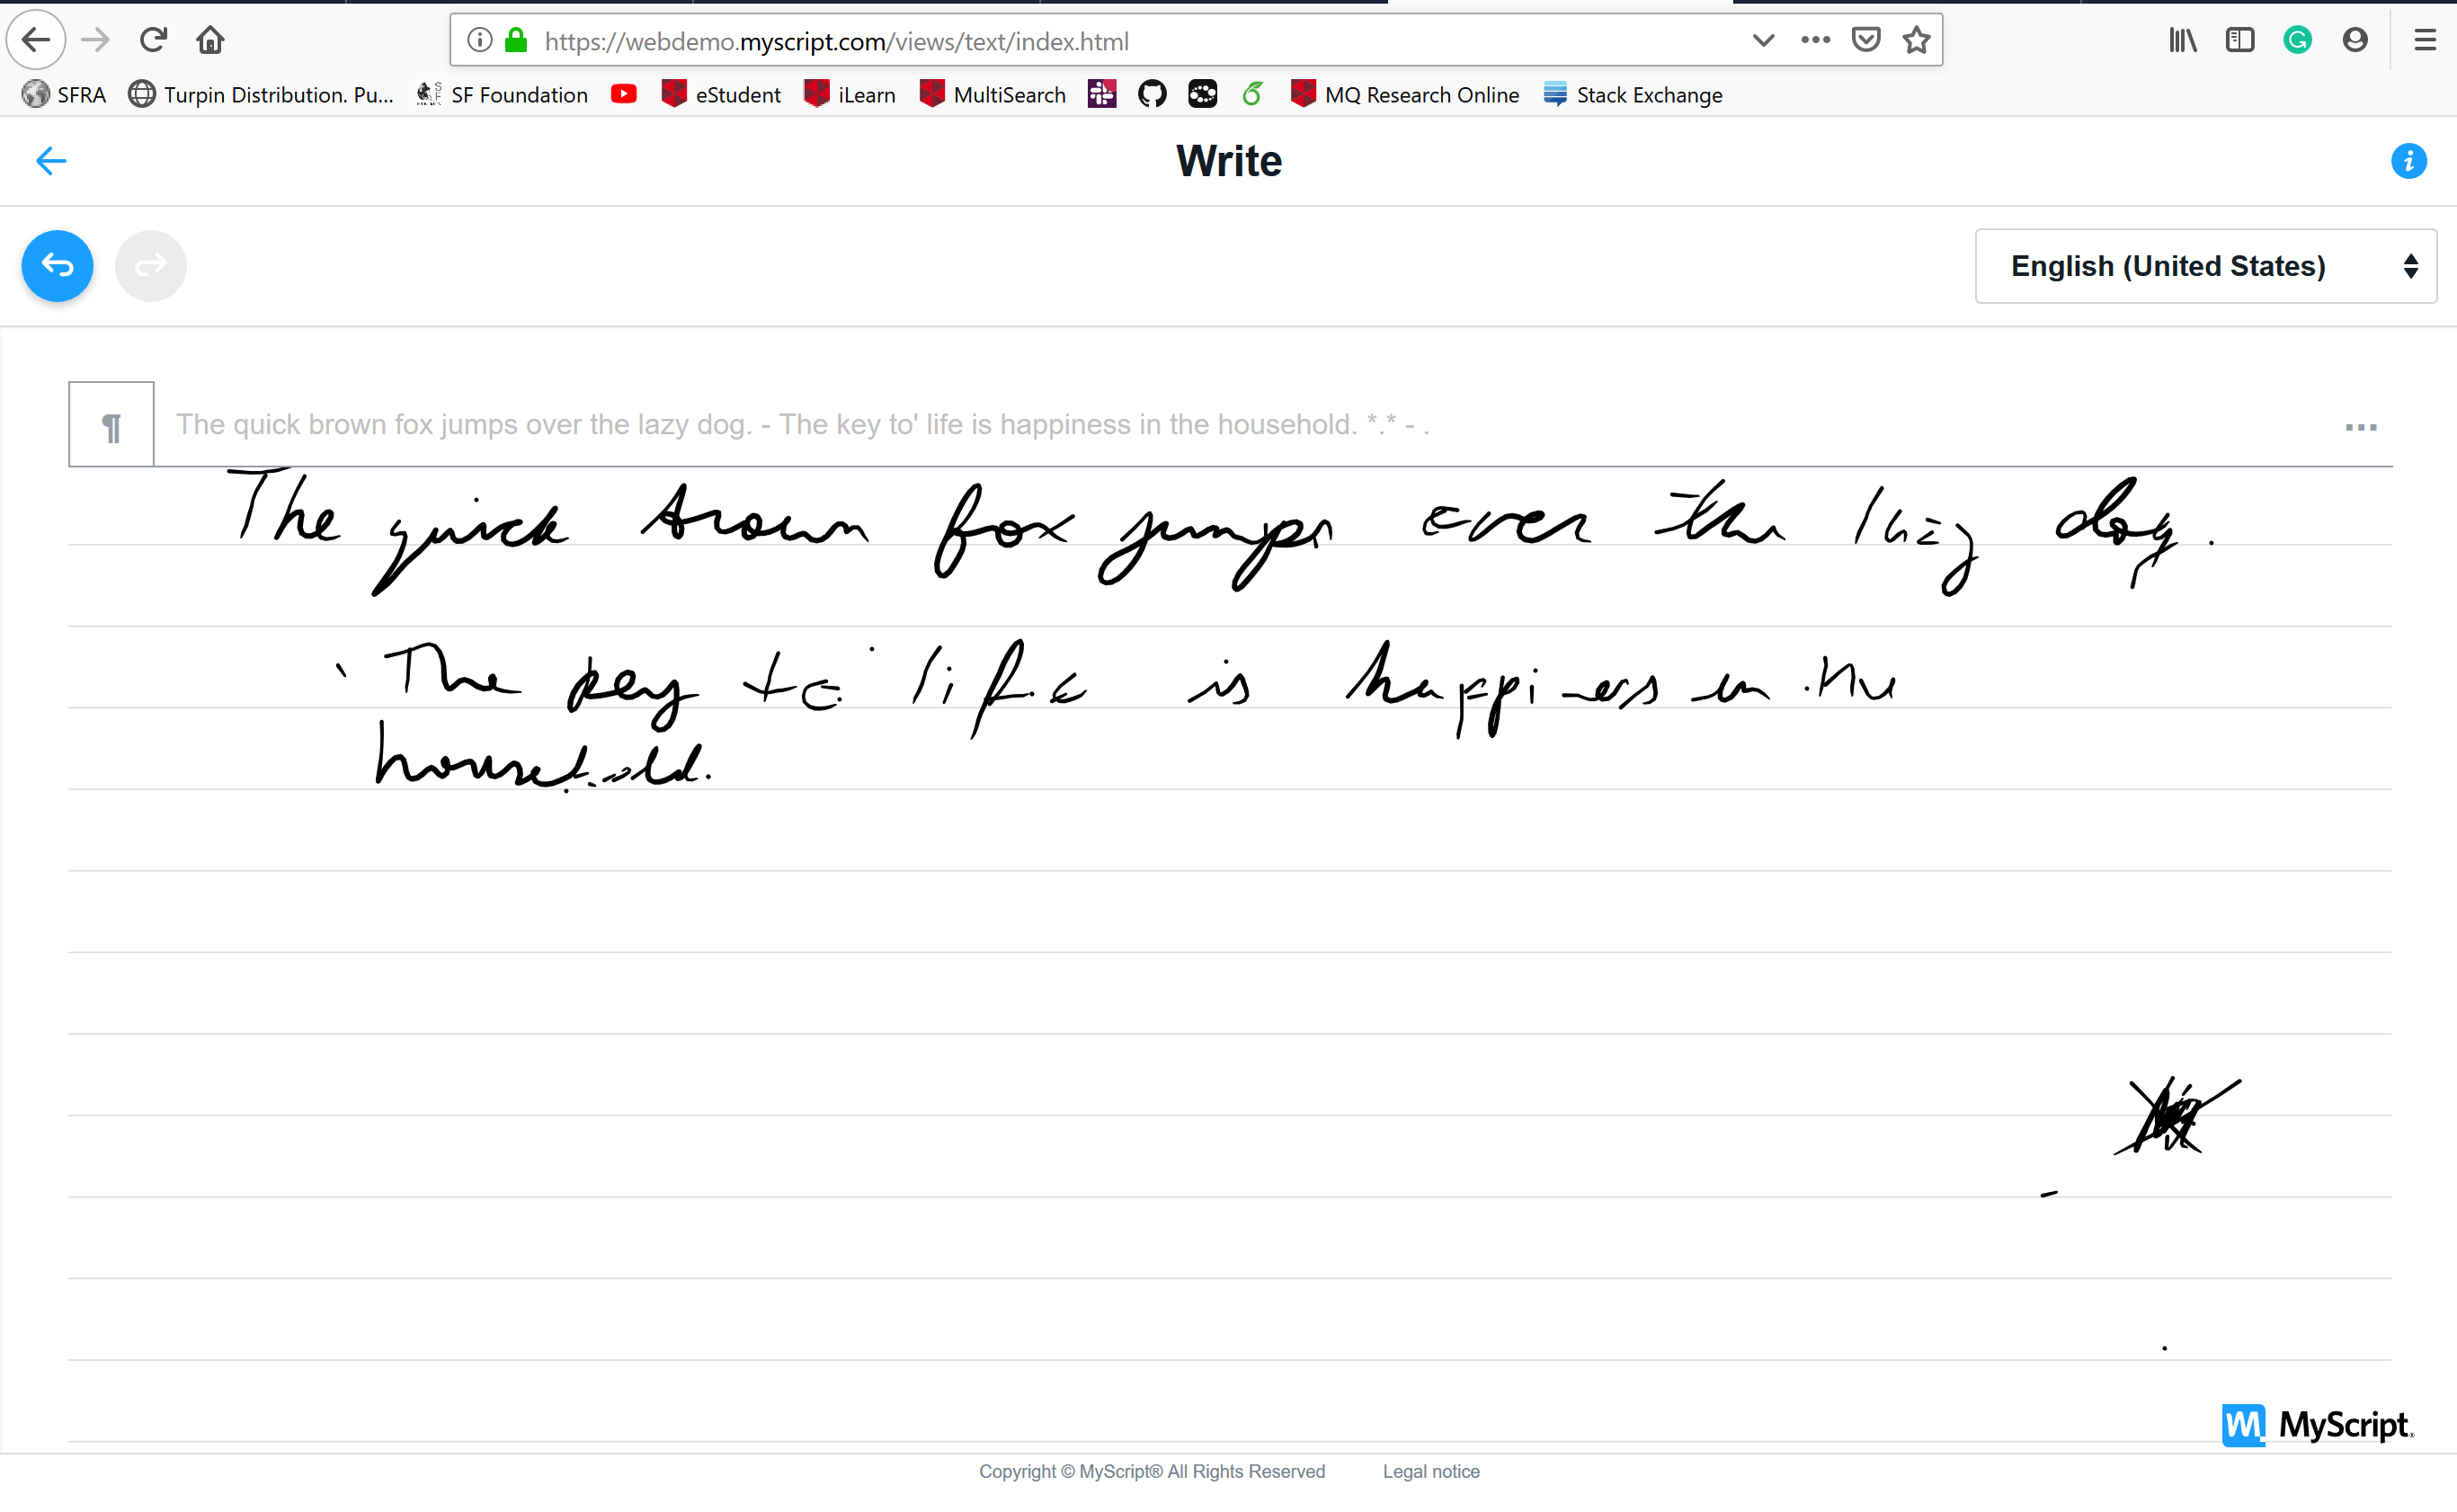
\includegraphics[width=11cm]{Images/NeboTest001.PNG}
    \caption{Testing the Nebo Interactive Ink WebApp Demo}
    \label{fig:Nebo Interactive Ink WebApp}
\end{figure}

\begin{figure}
    \centering
    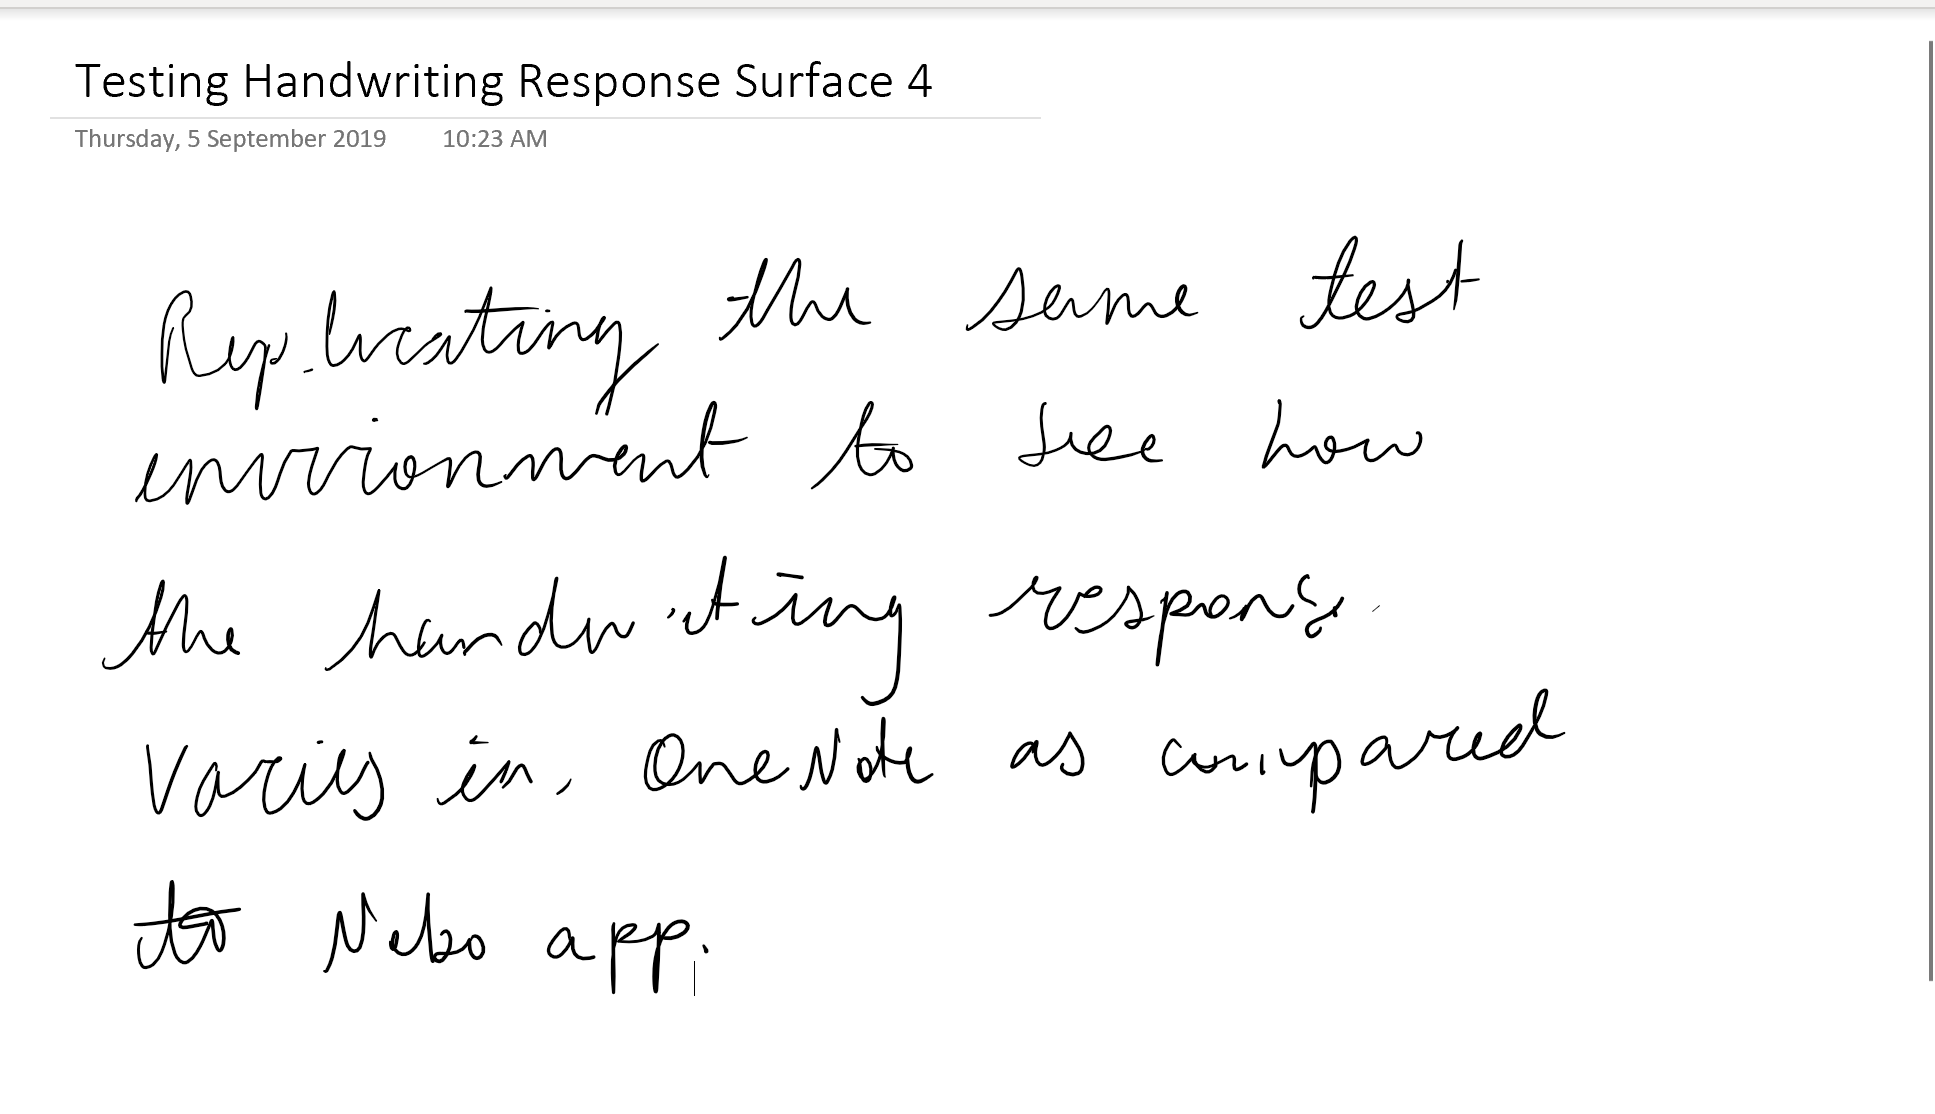
\includegraphics[width=11cm]{Images/OneNoteTest001.PNG}
    \caption{Testing handwriting in OneNote as a comparison to Nebo Interactive Ink}
    \label{fig:OneNote Handwriting}
\end{figure}
\textbf{Useful Links}

https://developer.myscript.com/text

https://webdemo.myscript.com/views/text/index.html

\textbf{Conclusion}

The Nebo Interactive Ink product has potential as a complementary digital note taking resource. It seems that it will require some calibration, and adjustment to my process, but nonetheless is a valid alternative to typed notes, and handwriting.

There is an API available - although as it is a paid software that is limited to developers, and access may be restricted. However at this stage, I am unsure if utilising the API for this software is necessary to the flow of my project. 


\subsection{Scrivener}

Scrivener is a software designed for writers to aid in orgnaising large-scale written projects. It has different default templates, and the ability to customise them, or create your own. Within the program there are spaces for distraction free writing, as well as research organisation. 

It is possible to get a 30-day (non-consecutive) free trial of the software, which is a full version. Which is excellent. It is also available across Mac and Windows platforms. It has an Apple App, but not an Android one at this stage - but there is one in development.

The price of this software is currently: 

\begin{itemize}
    \item AU \$69 for Standard Windows Licence
    \item AU \$77 for Standard macOS Licence
    \item AU \$19.99 for iOS (iPhone, iPad etc)
\end{itemize}

\textbf{Aim:}

I have purchased this software previously, and used it for creative works, however in this test, I will be exploring its capacity for organising academic research.

\textbf{Resources:}
\begin{itemize}
    \item Scrivener for Windows. Version: 1.9.13.0 (last updated 25 July 2019)
\end{itemize}

\textbf{Expectation:}
I hope to be able to import documents into Scrivener to be able to view them easily while completing work related to them. I would also like to find out how I am able to organise the documents, and if I can apply my own searchable tags to the documents.
Ideally I want to be able to:
\begin{itemize}
    \item Drag files from a directory on my computer to Scrivener for organisation/tagging
    \item Be able to organise files in a logical and flexible way - flexible meaning I can change structure relatively easily, and can apply different forms depending on the type of writing project.
    \item Apply/add searchable tags/keywords to files/documents.
\end{itemize}


\label{Error: Scrivener Errors/Frustrations}
\textbf{Errors/Frustrations:}

\begin{outline}
\1 I first created a blank Scrivener project - without utilising any of the pre-set ``project types''. 
    \2 The sections Draft, Research, and Trash are automatically created. 
\1 I go to the Research section and drag a pdf file from a File Explorer window onto the corkboard.
    \2 An index card is made for the file, and I am able to enter my own text onto the card. Clicking on the filename in the left hand 'binder' brings the file to the screen within scrivener. 
\1 I try the dual window function:
    \2 I am able to bring different things to each screen in Scrivener. I am able to bring the document to one screen, and have the corkboard with index card on the other. This is useful for writing the citation information down. 
\1 I try dragging a word document:
    \2 Scrivener ``reads'' the document and makes it into an editable document within Scrivener. 
\1 I want to add a folder to the ``binder'':
    \2 I use right mouse click on Research. This allows me to add a folder. I try using ctrl + n, and this creates a new document within the folder. If I do this with Research selected, it creates a new document in that folder. 
\1 Organising Folders
    \2 I am able to bring the newly created folder to one screen, and Research in the other. With both in corkboard view, I am able to drag index card from one to the other to move how the files are organised hierarchically.
\1 Adding searchable Labels/Keywords
    \2 I am able to apply a ``label'' to an index card/associated document. To do this I must create the label first, and then select it to apply it to the index card. This is great for controlling the vocabulary, and not having multiple variations of the same label. I am only able to apply one label to the index card though. Labels are coloured though, and so there is a nice aesthetic visual there. 
\1 Testing search functionality
    \2 When testing the search function I tested few terms. 
    \2 I tested Posthumanist - which returned one result where the word appears on the front page of the pdf document
    \2 I tested Posthuman - which returned similar results. When I viewed the word document that Scrivener ``read'' and was able to make editable - it also highlighted the term within the document. It also returned the folder in Research by the same name, and all its contents, even though the contents may not include the term.
    \2 I tested Philosophers - which did not return any results, even though I know the term is used later in one of the pdf files.
\1 Changing files that have been moved to Scrivener
    \2 I found that once a file has been moved into the Scrivener environment it is isolated there. Changes I made to the word document in word, were not applied to the file that Scrivener had adapted. SO that is a one way process. Likewise changes made in Scrivener did not reflect back to the orginial word file - those were now specific to the version within Scrivener.
\end{outline}

\textbf{Conclusion:}

I found that Scrivener was more useful for research that I imagined it to be, despite it following a very similar (and very useful) structure of operations in the draft/writing side. 
I was able to accomplish about half of the things I set out to do, in the way I wanted to do them. Some of the other functions, and not available, but may be adaptable. So I will be exploring the backend of Scrivener more, and seeing if there are suitable modifications or work-arounds that can be applied.

\begin{figure}[htbp]
    \centering
    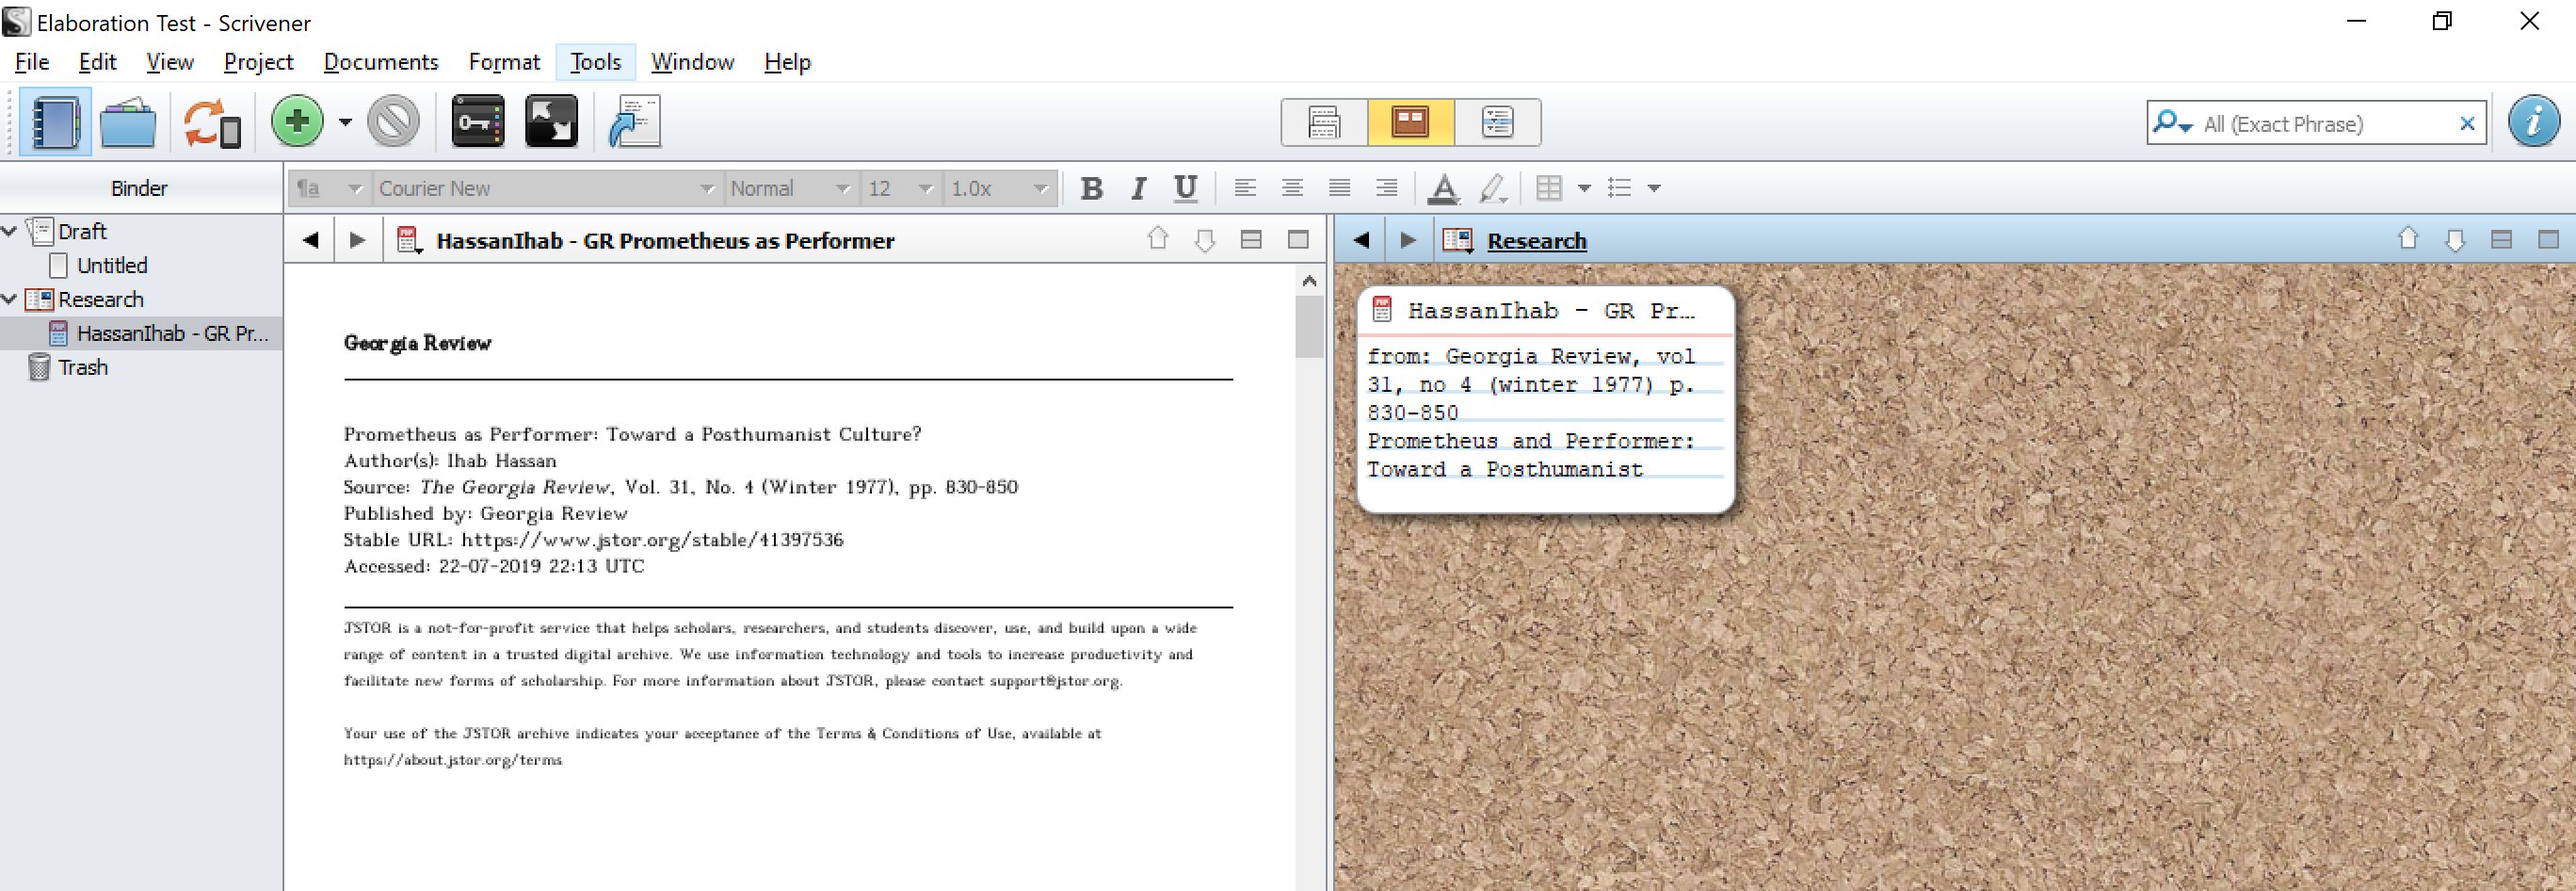
\includegraphics[width=11cm]{Images/ScrivenerTest001.PNG}
    \caption{Importing files into Scrivener}
    \label{fig:Scivener Research Screen}
\end{figure}

\begin{figure}[htbp]
    \centering
    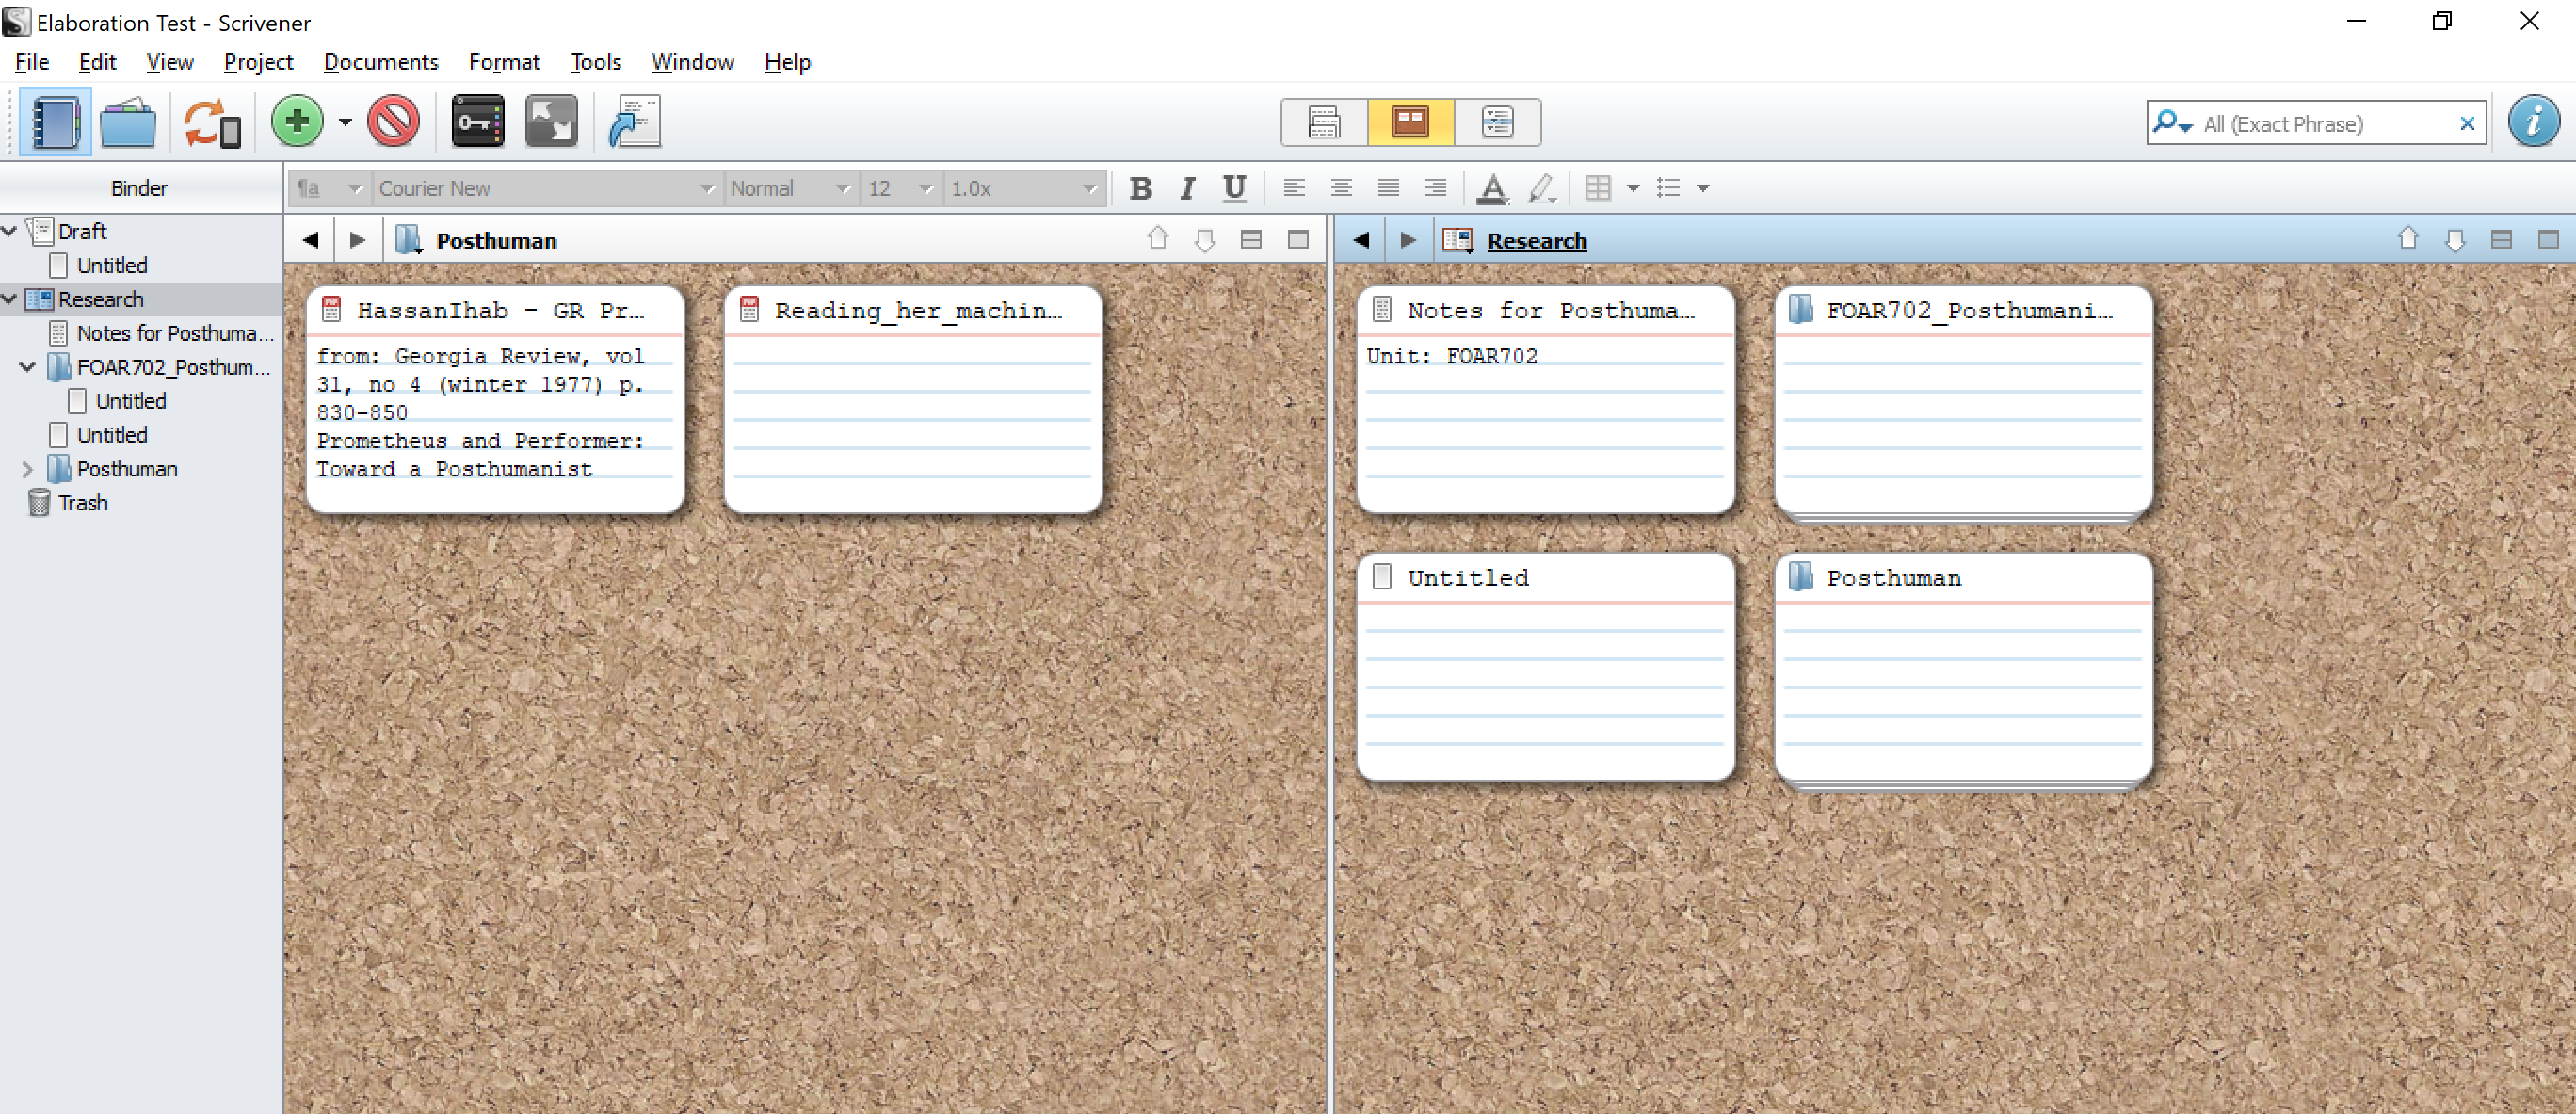
\includegraphics[width=11cm]{Images/ScrivenerTest002.PNG}
    \caption{Organising folders by dragging Index Cards}
    \label{fig:Scrivener Folder Organisation}
\end{figure}

\begin{figure}[htbp]
    \centering
    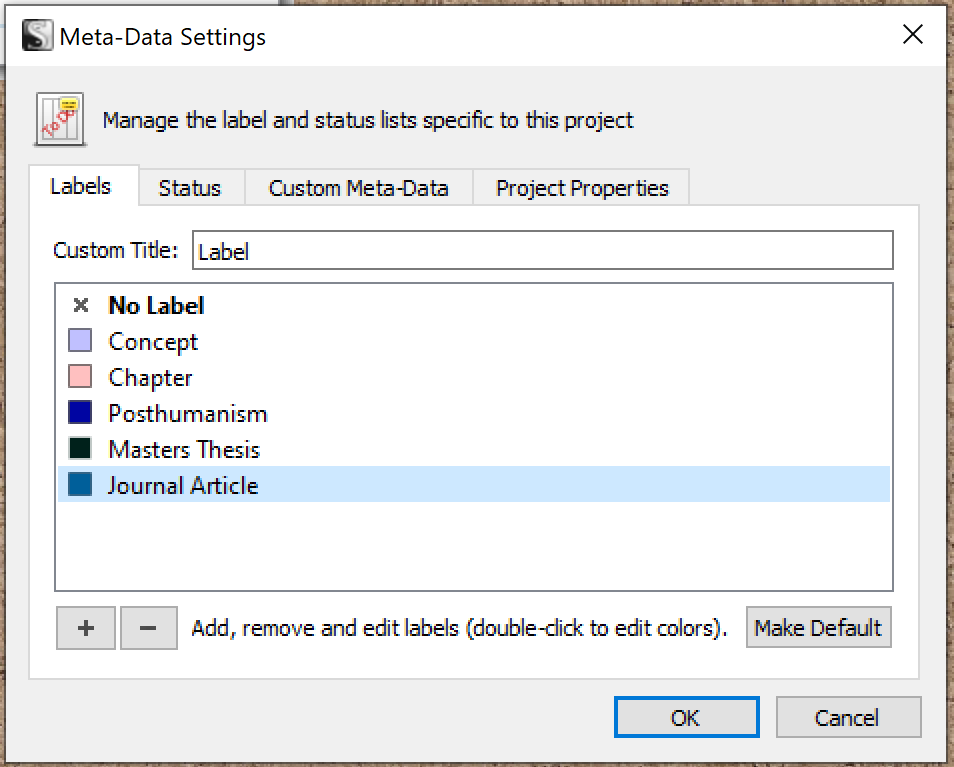
\includegraphics[width=8cm]{Images/ScrivenerTest003.PNG}
    \caption{Customizable labels in Scrivener}
    \label{fig:Scrivener Labels}
\end{figure}

\begin{figure}[htbp]
    \centering
    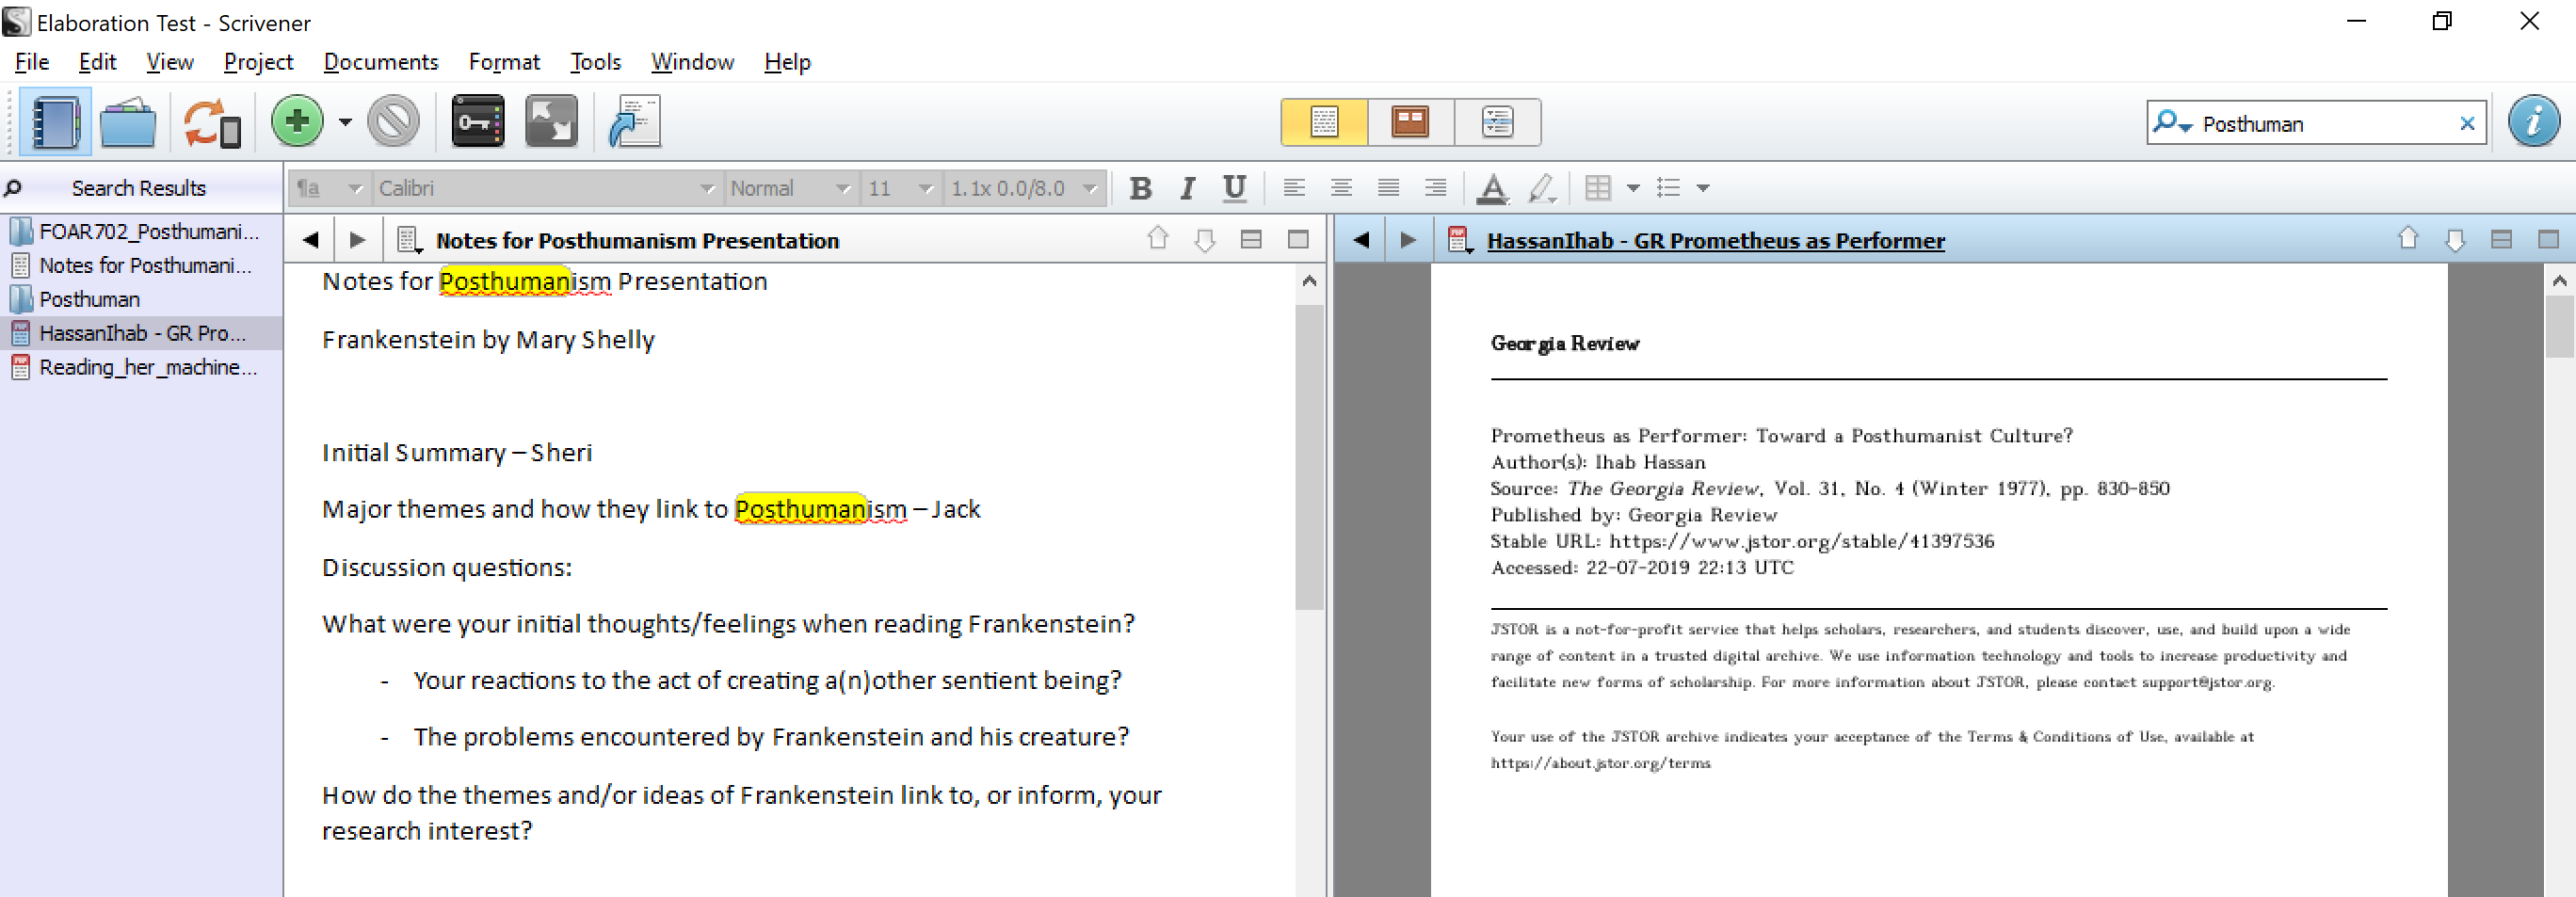
\includegraphics[width=11cm]{Images/ScrivenerTest004.PNG}
    \caption{Searching in Scrivener for Posthumanism}
    \label{fig:Scrivener Search Posthumanism}
\end{figure}

\begin{figure}[htbp]
    \centering
    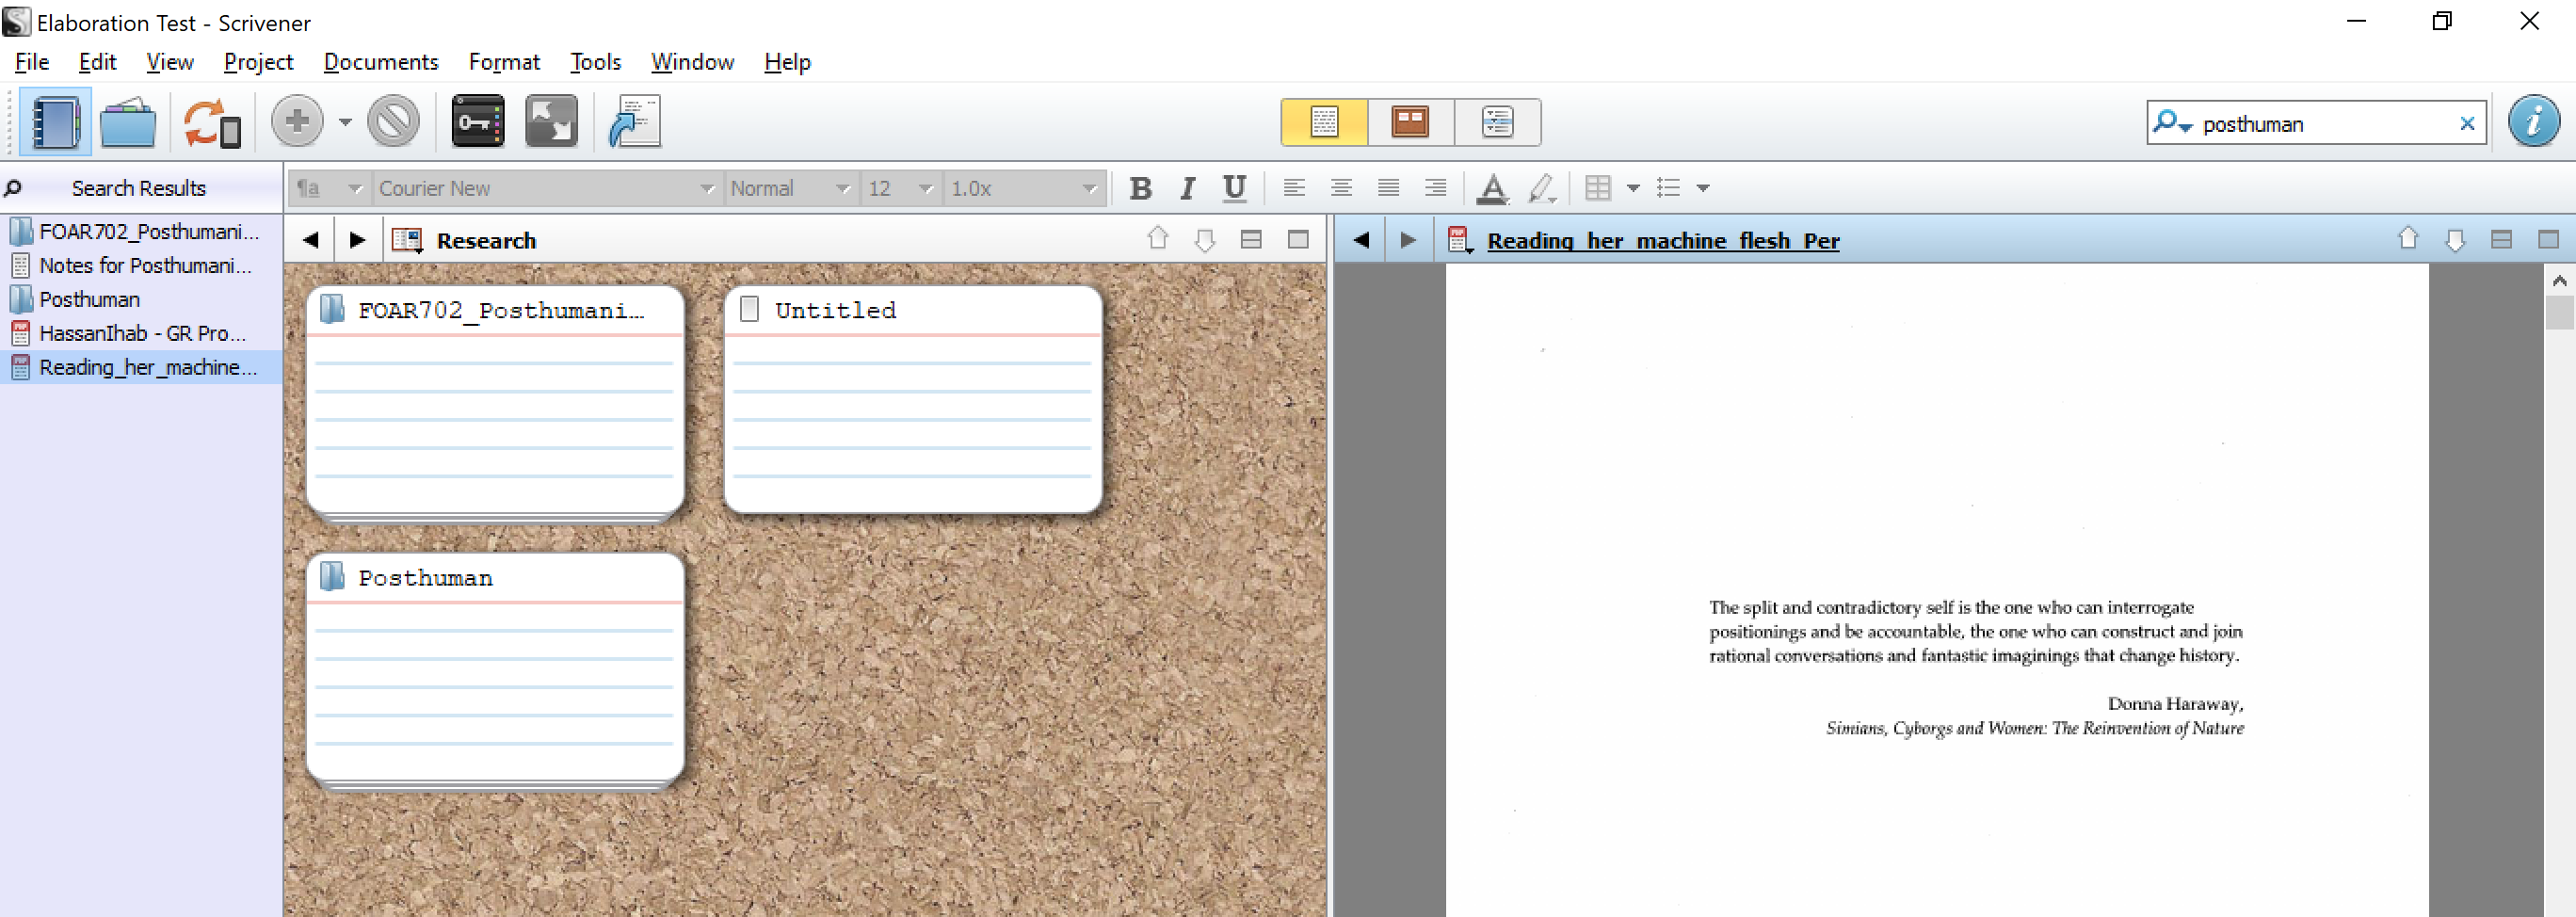
\includegraphics[width=11cm]{Images/ScrivenerTest005.PNG}
    \caption{Searching in Scrivener for Posthuman}
    \label{fig:Scrivener Search Posthuman}
\end{figure}

\begin{figure}[htbp]
    \centering
    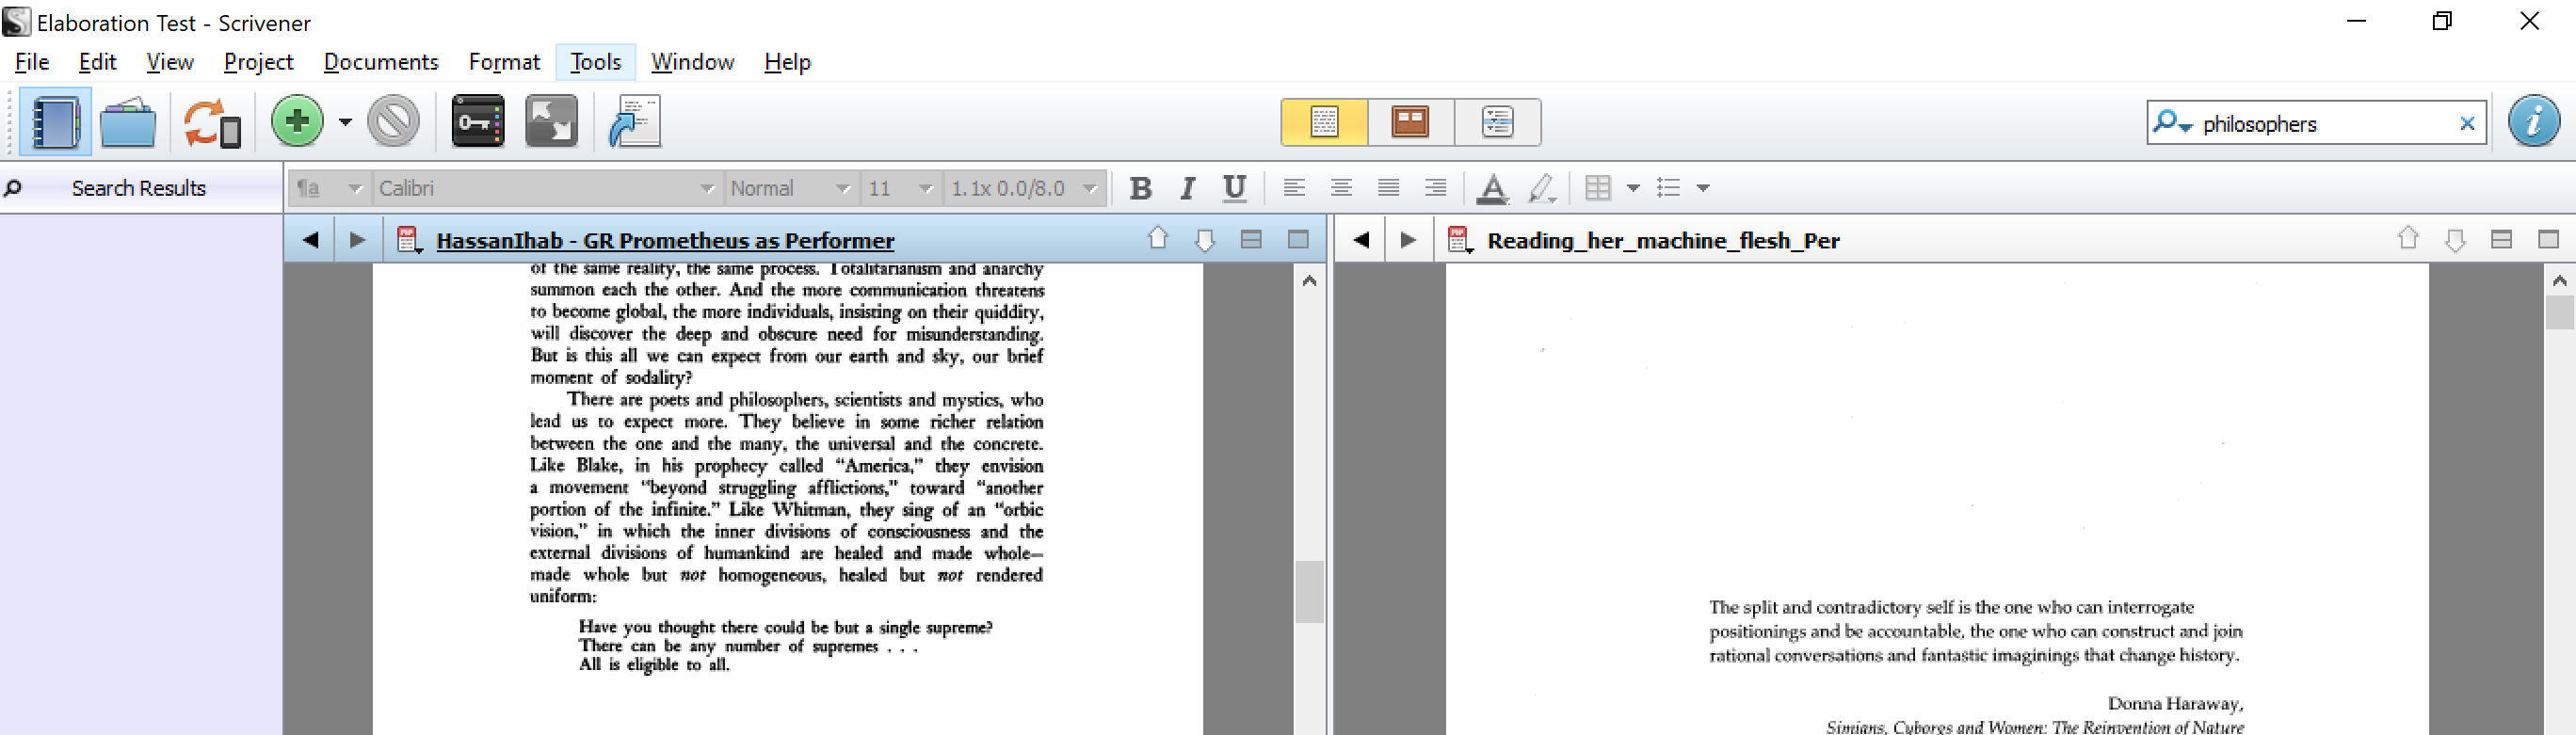
\includegraphics[width=11cm]{Images/ScrivenerTest006.PNG}
    \caption{Searching in Scrivener for Philosophers}
    \label{fig:Scrivener Search Philosophers}
\end{figure}

\pagebreak

\subsection{OneNote}

OneNote is a Microsoft porgram, and is included with Windows 10. It is available as a WebApp, and across macOs, iOS, and Android. 

\textbf{Aim:}


\textbf{Resources:}

OneNote as issued with Windows 10 on my Microsoft Surface 4.

I have used OneNote for general note-taking, and its availability across platforms, and its connectivity to OneDrive have been very useful. All information within OneNote though is stored in a cloud that is controlled by Microsoft. 

\textbf{Expectation:}

I hope to be able to import documents into OneNote to be able to view them easily while completing work related to them. I would also like to find out how I am able to organise the documents, and if I can apply my own searchable tags to the documents.
Ideally I want to be able to:
\begin{itemize}
    \item Drag files from a directory on my computer to OneNote for organisation/tagging
    \item Be able to organise files in a logical and flexible way - flexible meaning I can change structure relatively easily, and can apply different forms depending on the type of writing project.
    \item Apply/add searchable tags/keywords to files/documents.
\end{itemize}

\label{Error: OneNote Errors/Frustrations}
\textbf{Errors/Frustrations:}

\begin{outline}
    \1 I created a new notebook called Elaboration, and renamed the first section to testing.
    \1 Dragging files to OneNote worked, and I was given options of how I wanted that file to appear in the note. 
        \2 Dragging a PDF, and selecting to "print" the file within the note took some time to process, but I ended up with a version of the file, that i was able to view directly in one note, and there is the option of typing/handwriting with a stylus. Notes with the stylus, can run over the document too. as it is treated more like an image.
        \2 Text that is typed next to the document is in text boxes, and these can overlap.
    \1 Organising files
        \2 I can manually order the notes within the section of the notebook, and I am able to order sections by clicking and dragging them. I am able to move pages between sections by clicking and dragging.
        \2 I am not able to have a summary view like in Scrivener with the corkboard.
    \1 Adding tags/keywords
        \2 I am not able to add tags/keywords as metadata to a note it seems.
        \2 when I opened the search menu, it has a tags result tab, so I investigated.
        \2 There is a way to add tags to a note in OneNote - as outline on this Microsoft Support \href{https://support.office.com/en-us/article/apply-a-tag-to-a-note-in-onenote-908c7b92-6ed0-498d-bc7d-1b44e6827d05}{page}.
        \2 I am able to add multiple tags to a single note, but it is not fixed as to where they are linked. It is dependant on where the cursor is when it is applied - So it can be in the heading, in the body, attached to an attachment. Which is potentially useful, but also potentially difficult to use/manage.
        \2 When adding the tags, they are added in a controlled manner, and can be associated with a limited range of icons. Tags are program wide, and not limited to a specific project the way labels are in Scrivener.
    \1 Searching
        \2 Search is across all notebooks
        \2 the terms are highlighted in the results
        \2 imported documents are not searched
        \2 tags can be searched/used to group notes in a transient way
    \1 Changing files that have been moved to OneNote
        \2 If a file is added to OneNote as an atachement or in-document print view, changes made to the original do not affect the document in OneNote. But if the document is linked from OneDrive, and the changes are made to the file in OneDrive - but through a different program, eg word, or ms paint, those changes will be visible. As it is a linked document, instead of a copy/stored document.
\end{outline}

\textbf{Conclusion:}

OneNote has proven to be a useful note-taking tool, however it is limited in its organisation capabilities. It is less rigid than Scrivener in some aspects, it is multi-platform, and syncs across devices, but it is less organisable, compared to Scriveners corkboard, and internal document view. Scrivener has split screen viewing, which OneNote does not.

\begin{figure}[htbp]
    \centering
    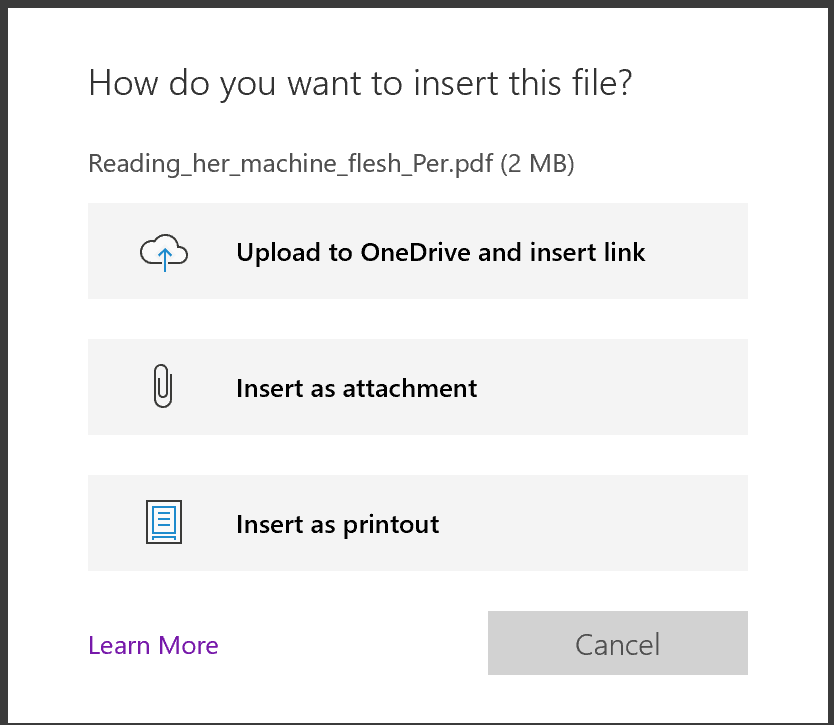
\includegraphics[width=11cm]{Images/OneNoteTest004.PNG}
    \caption{Options for imported file appearance in OneNote}
    \label{fig:OneNote File Import}
\end{figure}

\begin{figure}[htbp]
    \centering
    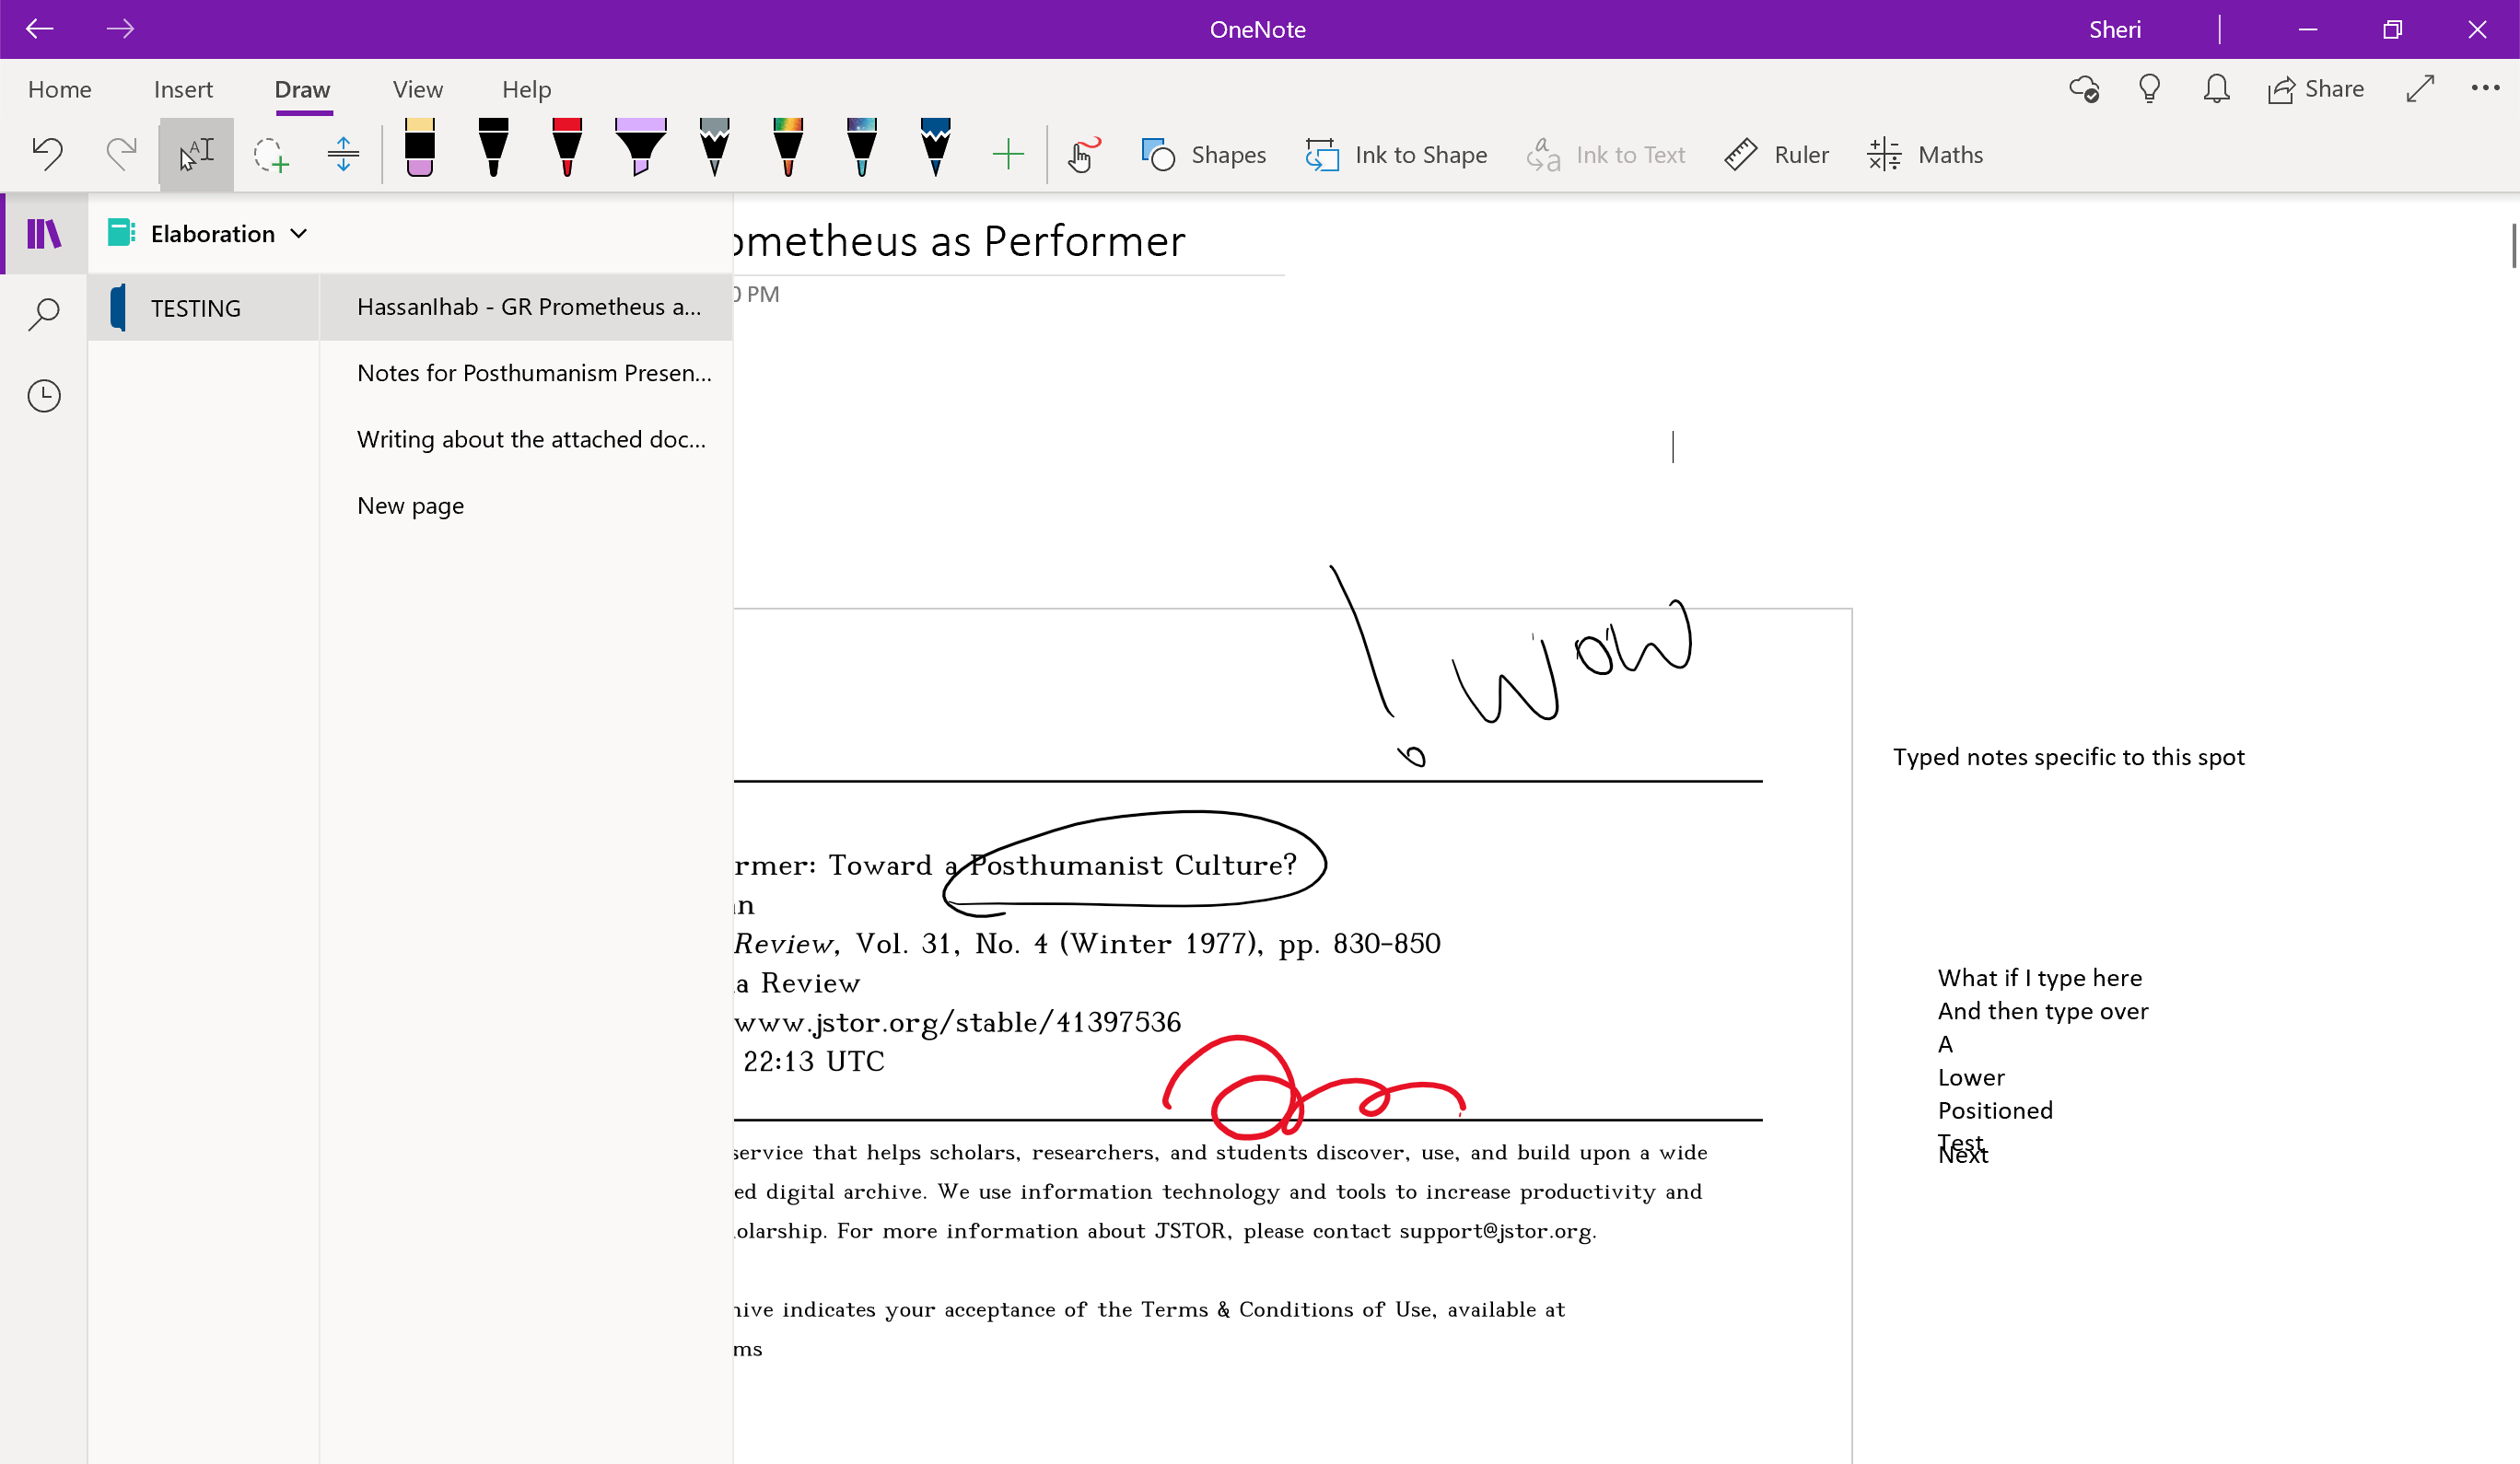
\includegraphics[width=11cm]{Images/OneNoteTest006.PNG}
    \caption{Notes around imported file - as print in note}
    \label{fig:OneNote Note Flexibility}
\end{figure}

\begin{figure}[htbp]
    \centering
    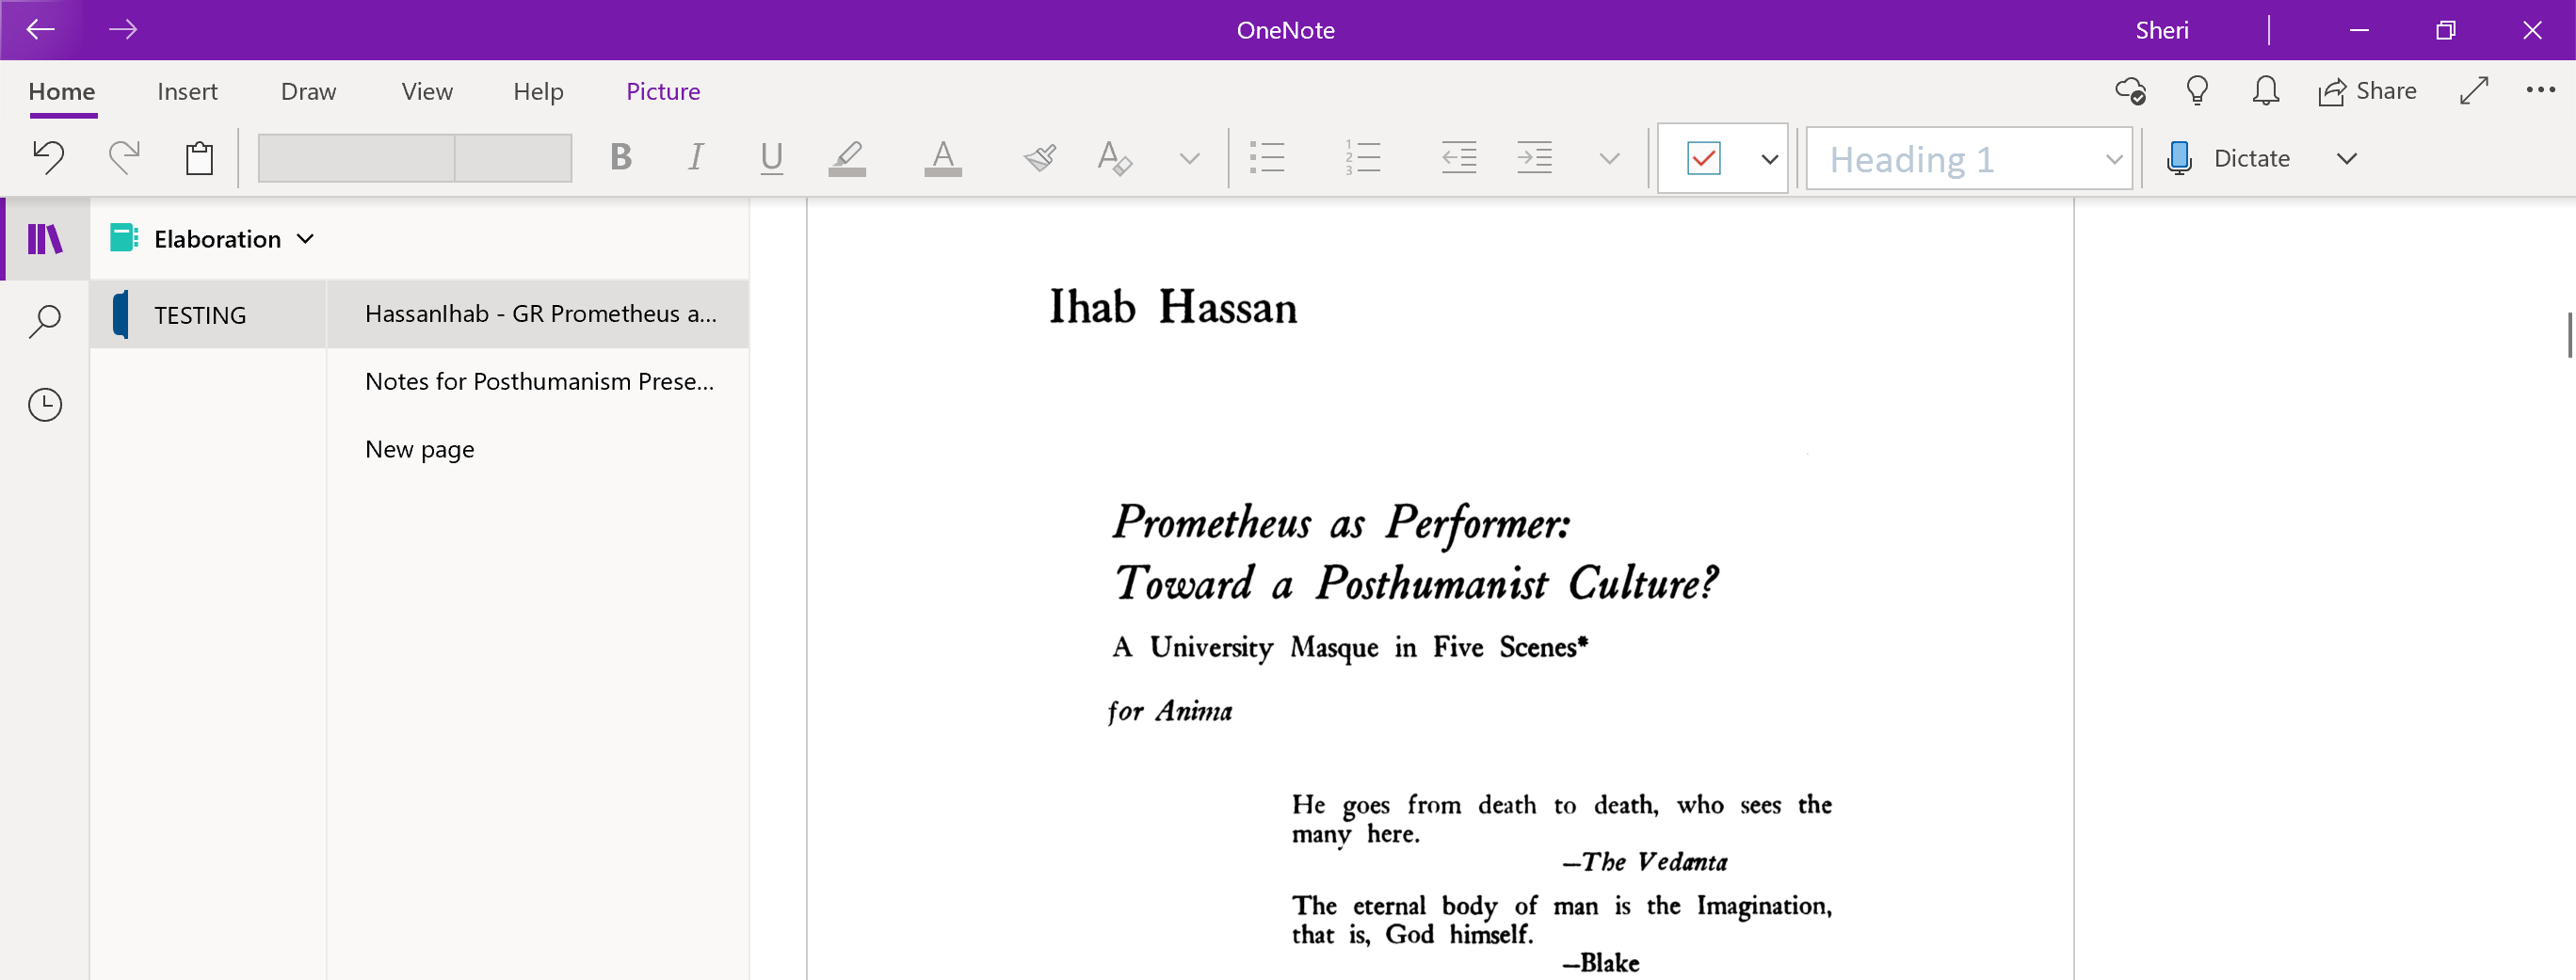
\includegraphics[width=11cm]{Images/OneNoteTest002.PNG}
    \caption{Creating Notebooks, sections, and notes in OneNote}
    \label{fig:OneNote Structure}
\end{figure}

\begin{figure}[htbp]
    \centering
    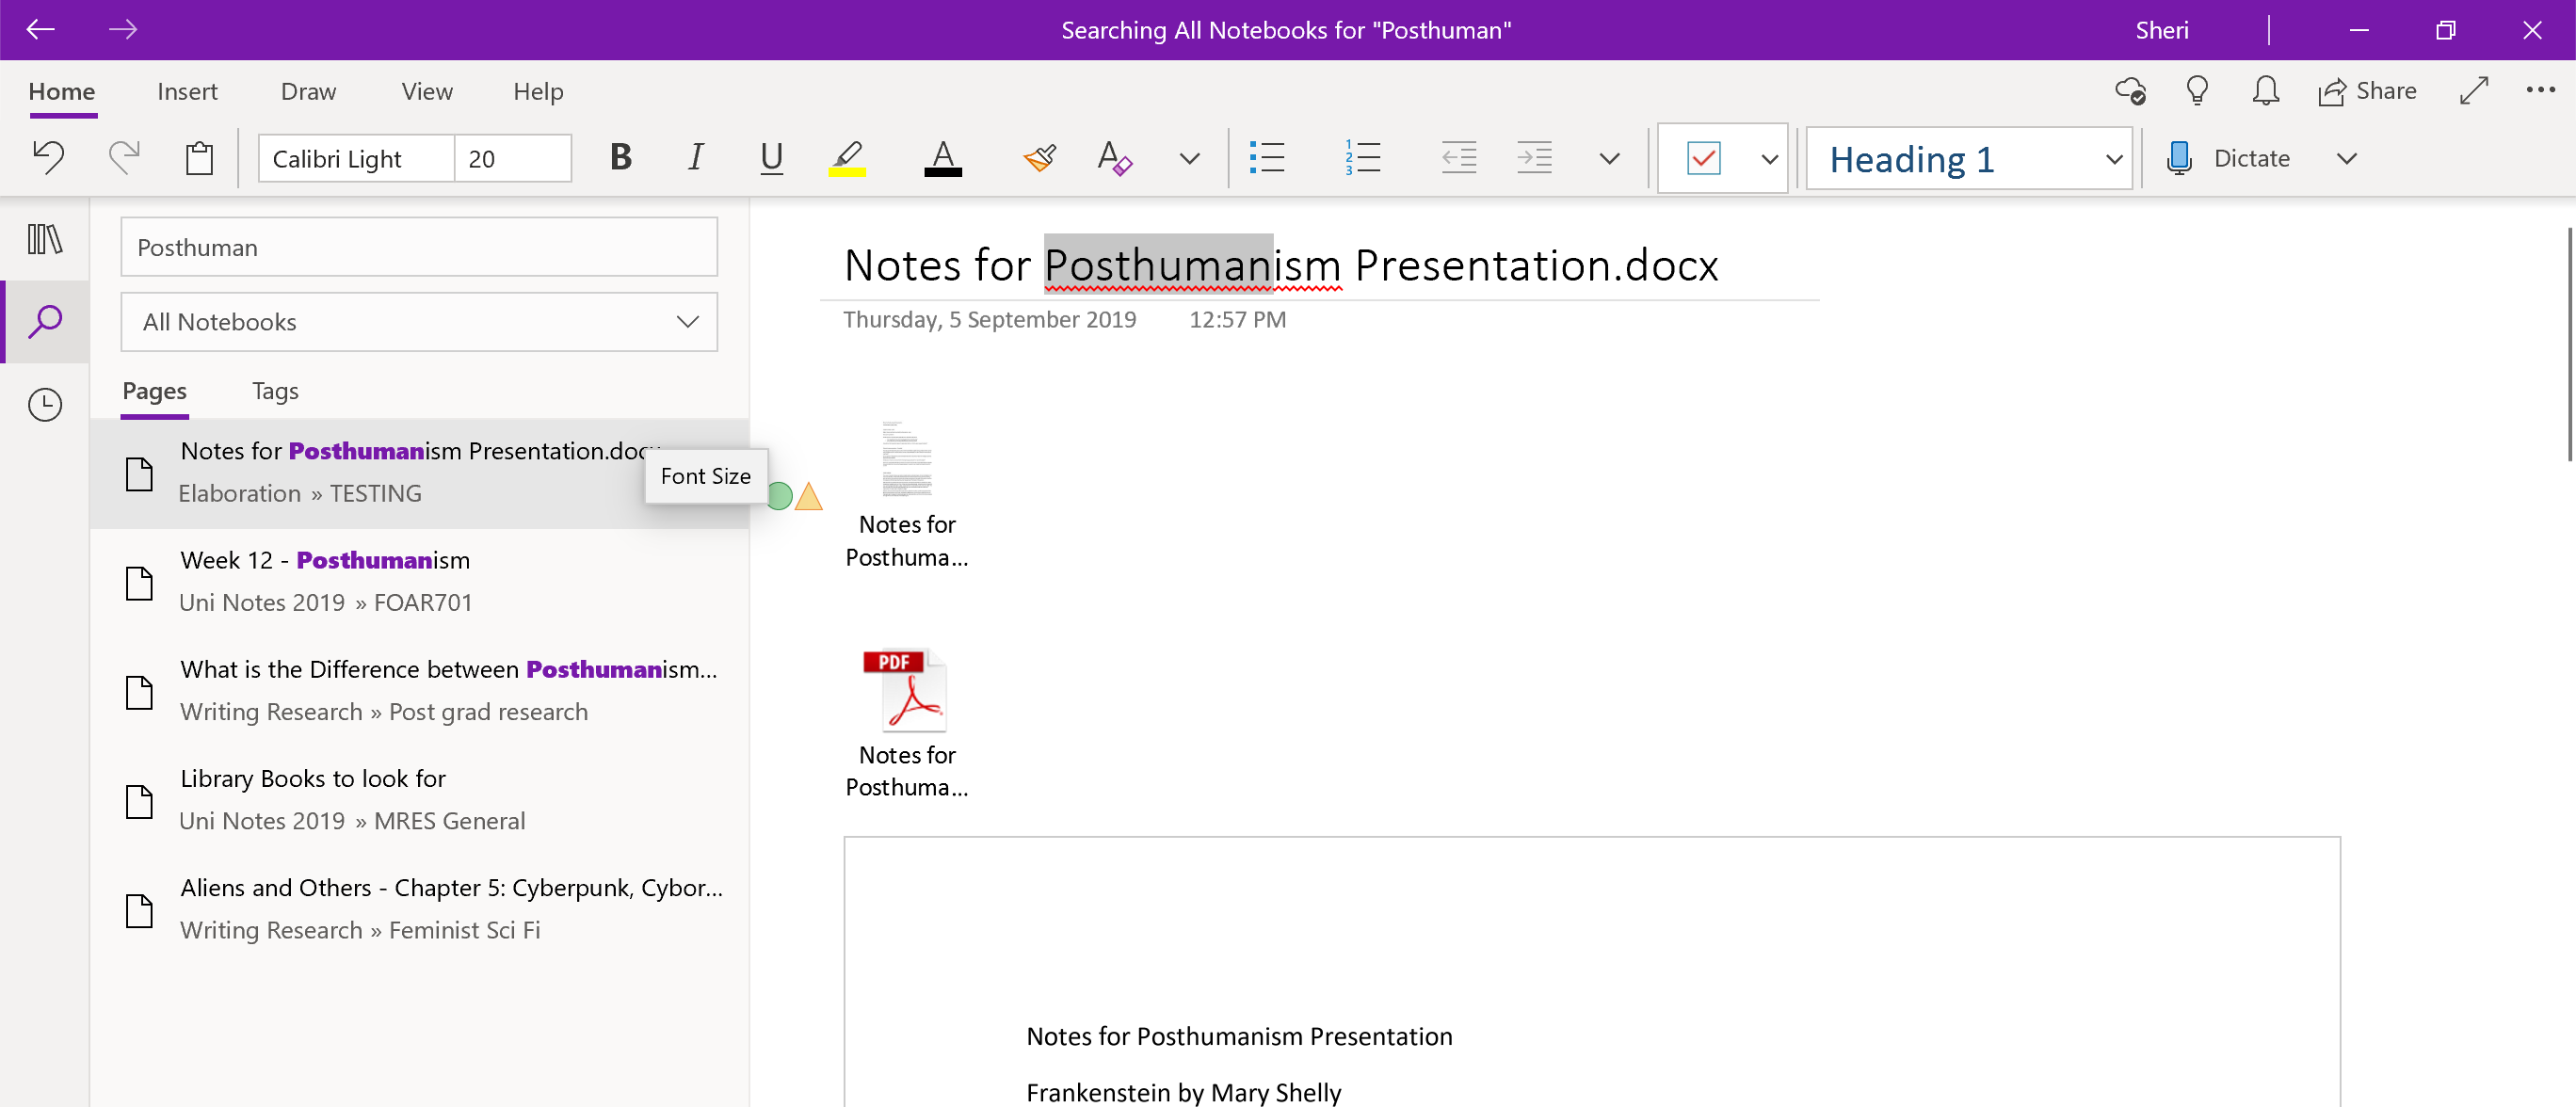
\includegraphics[width=11cm]{Images/OneNoteTest003.PNG}
    \caption{Searching for term Posthuman in OneNote}
    \label{fig:OneNote Search Posthuman}
\end{figure}

\begin{figure}[htbp]
    \centering
    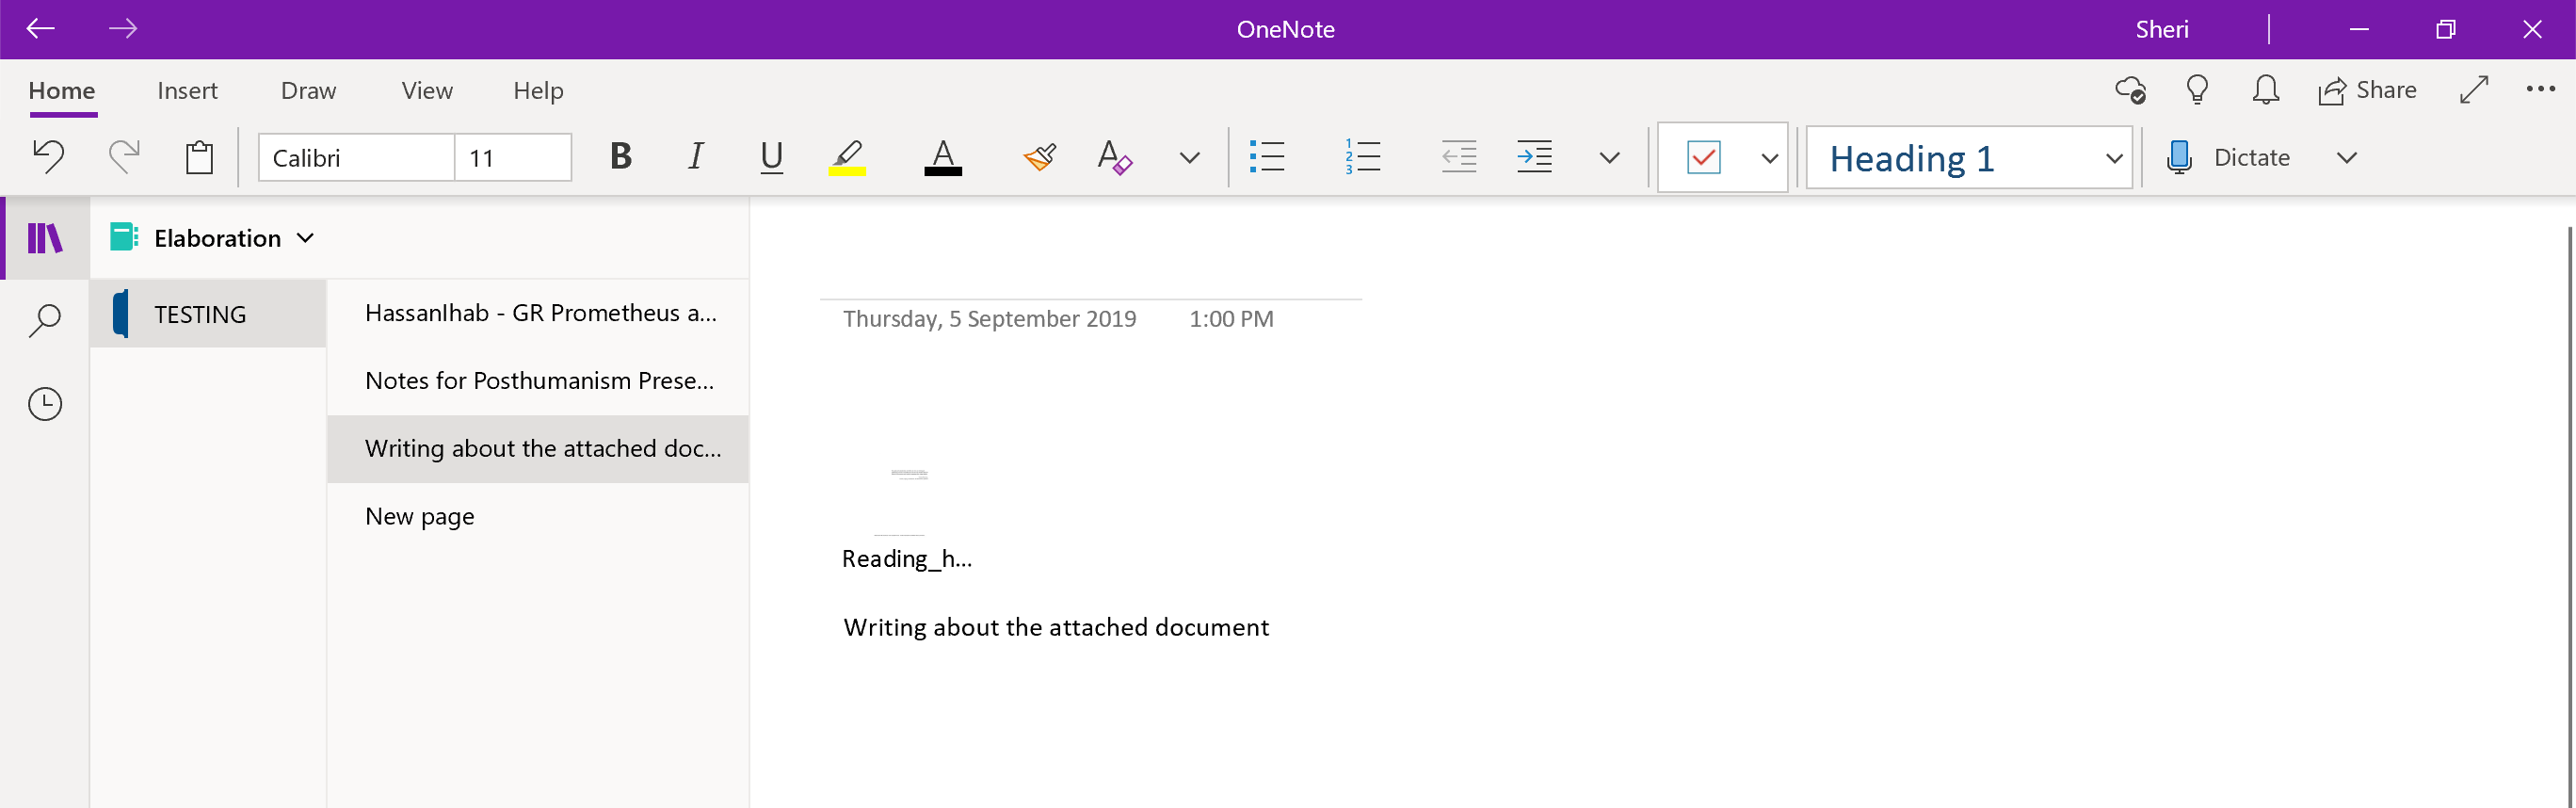
\includegraphics[width=11cm]{Images/OneNoteTest005.PNG}
    \caption{Caption}
    \label{fig:my_label3}
\end{figure}

\pagebreak

\subsection{Zim}

Zim is a graphiacal text editor. It is an opensource software. It was inspired by the way people use wikipedia.

It was reccomended as a windows friendly alternative to DevonThink, which is a macOS based DMS. 

\textbf{Aim:}

To install and run Zim, and test it for usefulness as a note taking, and document management tool.

\textbf{Resources:}
\begin{itemize}
    \item https://www.zim-wiki.org/
    \item Installer for windows - https://zim.glump.net/windows/
\end{itemize}

\textbf{Expectation:}

I hope to be able to import documents into Zim to be able to view them easily while completing work related to them. I would also like to find out how I am able to organise the documents, and if I can apply my own searchable tags to the documents.
Ideally I want to be able to:
\begin{itemize}
    \item Drag files from a directory on my computer to OneNote for organisation/tagging
    \item Be able to organise files in a logical and flexible way - flexible meaning I can change structure relatively easily, and can apply different forms depending on the type of writing project.
    \item Apply/add searchable tags/keywords to files/documents.
\end{itemize}

\label{Error: Zim Errors/Frustrations}
\textbf{Errors/Frustrations:}

\begin{outline}
\1 Installing Zim
    \2 Zim is an opensource software, and so it's code and so on is freely available and editable. There is a github repository at: \url{https://github.com/zim-desktop-wiki/zim-desktop-wiki}
    \2 I use a widows installer to install the most recent version of Zim, and run the program.
\1 Notebook creation.
    \2 when i first run Zim, I must create a notebook.
\1 Document creation
    \2 control + n creates a new page
\1 Dragging files to Zim
    \2 I am not able to drag a file to Zim, and have Zim recognise it and process it automatically in any way.
    \2 I am able to ``attach'' files, which creates a link to them. This has potential to be useful when writing on/about specific papers. 
    \2 clicking the link/attachment opens the file in its native form, so adobe reader for .pdf, or Word for .doc. This means that changes to the original will flow through to what the link accesses.
\1 Organising Files
    \2 as the files are attached to single pages, this is note a useful tool for organising data, like journal articles, my own notes, or other documents, in a way that can be networked automatically.
\1 Adding tags/keywords
    \2 I am unable to find a way to add tags or searchable keyworods to a page in Zim. However as it is an opensource and communty driven program - it is highly likely that something exists that enables this beyond the basic installation. 
    \2 \url{https://github.com/jaap-karssenberg/zim-wiki/wiki}
\1 Searching
    \2 When searching in Zim, it is not able to search the contents of linked documents - only the filename as it appears in the link, and the content that has been directly entered into Zim.
\end{outline}

\textbf{Conclusion:}

The basic install of Zim DesktopWiki is not sufficient for my needs, but there is great potential that there will be adaptable solutions in the community driven developments. 

Sifting through this information to find what will best suit my needs will require knowledgeable assistance.

\pagebreak

\section{Testing Data Synthesis and Mapping}

\subsection{Miro}

Miro is a team collaboration software. 
It does charge for licensing if it is going to be used by more than one person within an organisation. But for a single user/personal account it is free.

\textbf{Aim:}

To test the capabilities of Miro as a mind mapping software, and potentially as a data visualisation tool.

\textbf{Resources:}
\begin{itemize}
    \item \url{www.miro.com}
    \item Miro Desktop App
\end{itemize}
\textbf{Expectation:}

\label{Error: Miro Errors/Frustrations}
\textbf{Errors/Frustrations:}

\textbf{Conclusion:}

\subsection{Scrapple}
\textbf{Aim:}

\textbf{Resources:}

\textbf{Expectation:}

\label{Error: Scrapple Errors/Frustrations}
\textbf{Errors/Frustrations:}

\textbf{Conclusion:}
\section{Testing Writing and Publication Software}


\subsection{ConTeXt}

\textbf{Aim:}

\textbf{Resources:}

\textbf{Expectation:}

\label{Error: ConTeXt Errors/Frustrations}
\textbf{Errors/Frustrations:}

\textbf{Conclusion:}

\subsection{BibTex}

\textbf{Aim:}

\textbf{Resources:}

\textbf{Expectation:}

\label{Error: BibTex Errors/Frustrations}
\textbf{Errors/Frustrations:}

\textbf{Conclusion:}

\subsection{Mendeley}

\textbf{Aim:}

\textbf{Resources:}

\textbf{Expectation:}

\label{Error: Mendeley Errors/Frustrations}
\textbf{Errors/Frustrations:}

\textbf{Conclusion:}


\end{document}
